\documentclass[UTF8,11pt,a4paper,openany,oneside]{ctexbook}
\usepackage{amsmath,amssymb,bm,graphicx,booktabs}
\usepackage[margin=27mm,headheight=15pt]{geometry}
\usepackage{hyperref}
\hypersetup{unicode=true,colorlinks=true,linkcolor=blue!45!black,urlcolor=blue!45!black,pdftitle={PHYS5120 计算物理中文自学教材}}
\usepackage{xcolor}
\usepackage{fancyhdr}
\raggedbottom
\pagestyle{fancy}
\fancyhf{}
\fancyhead[L]{\small 计算物理：从原子运动到电子结构}
\fancyhead[R]{\small\thepage}
\renewcommand{\headrulewidth}{0.3pt}
\setlength{\parskip}{0.35em}
\setlength{\emergencystretch}{2em}
\newcommand{\dd}{\mathrm{d}}
\newcommand{\ii}{\mathrm{i}}
\newcommand{\kb}{k_{\mathrm B}}
\newcommand{\Tr}{\operatorname{Tr}}
\newcommand{\sourcepages}[1]{\par\smallskip{\small\textit{资料对应：#1。}}\par\medskip}
\graphicspath{{figures/}}

\begin{document}
\frontmatter
\title{计算物理：从原子运动到电子结构\\\large PHYS5120 中文自学教材}
\author{课程笔记整理}
\date{2026 年 11 月}
\maketitle
\chapter*{致读者}
计算材料的性质，首先要回答三个问题：用什么变量描述材料，怎样求出这些变量的分布或运动，以及怎样判断计算结果可信。本书沿这三个问题展开。我们先把原子当作经典粒子，学习轨迹与平衡采样；再追问原子间的力从何而来，进入多电子量子力学；最后把电子结构方法用于晶体、振动和第一性原理分子动力学。

本书假设读者掌握微积分、向量与矩阵的基本运算。概率分布、变分、量子态及多体近似在需要时引入。第一次阅读时应沿章序前进：后面的算法依赖前面建立的物理模型，公式的适用范围与公式本身同样重要。

本稿依据原有课程协作笔记及朋友提供的 50 页手写笔记重新组织，以中文 LaTeX 为正文。教学原则取法 Cohen--Tannoudji《Quantum Mechanics》所体现的循序渐进、问题驱动与推导和物理解释相结合；文字与推导独立编写。原协作笔记贡献者的署名权益保留。手写资料是理解课程的线索，不能代替对公式的独立检查。本稿是可继续深化的中文教材初稿，而非已经完成同行评审的定稿。
\tableofcontents
\mainmatter
\section{Molecular dynamics}
\subsection{Basic statistical mechanics}
Consider a box consider N-partciles, we would like to study the property of this system. The particles in this system has interaction. In MD, we have a force field and the field here depends on position. In this course, we mainly only consider the Coulomb's interaction:
\begin{equation}
    F=k\frac{q_1 q_2}{r^2}
\end{equation}

The approach in classical mechanics includes:\\
1. Newton's equation of motion,

\begin{equation}
    \textbf{F}=m\frac{d^2 \textbf{x}}{dt^2}
\end{equation}

2: Hamiltonian mechanics.
\begin{equation}
    \dot{\hat{p}}=-\frac{\partial H}{\partial q}
\end{equation}
\begin{equation}
    \dot{\hat{q}}=\frac{\partial H}{\partial p}
\end{equation}

3: Lagrangian mechanics

If we want to describe a state, we can have a state point, where the state function $S=(q,p)=(r_1,r_2,...,r_N,p_1,p_2,...,p_N)$. The phase space of the system has $6N$ dimension.

\subsubsection{NVE ensemble}
In NVE ensemble system, the number of particle(N), volume(V), and Energy(E) is unchange in the system. The expected value of A (such as pressure) can be written as:
\begin{equation}
    <A>=\frac{\sum_S\delta_{\varepsilon(S),E} A(S)}{\sum_S \delta_{\varepsilon(S),E}}
\end{equation}
\subsubsection{Canonical ensemble/NVT}
If the Temperature of the system is confined instead of energy, we will have the NVT ensemble.
\begin{equation}
    <A>=\frac{\sum_S e^{-\beta \varepsilon(S)} A(S)}{\sum_S e^{-\beta \varepsilon(S)}}
\end{equation}

Classically, we can define temperature as
\begin{equation}
    \sum^N_{i=1} \frac{\textbf{p}_i^2}{2m} = \frac{3Nk_BT}{2}
\end{equation}
\subsection{Ergodicity}
The Ergodic hypothesis means that the ensemble average can be obtained by the time average:

\begin{equation}\label{eqn:Ergodicity}
    <\textbf{A}>=\lim_{t\rightarrow\infty}\frac{1}{t}\int_0^\infty dt' \textbf{A}(t')
\end{equation}

In MD, the hypothesis means that if the simulation, equation \eqref{eqn:Ergodicity} will give us an accurate results. This works for fluids, supercritical fluids, or gas, but does not work for solid and glass.

\subsection{Molecular Dynamics (MD)}
To perform MD, we need 1. State function $S_i$, and 2. $F_i$: There are two types of Force field $F_i$, including classical MD, and quantum mechanics MD (first-principles MD, or ab initio MD). 3. Given a time steps h, we solve the equation motion of $t\rightarrow t+h$. Step 2 and Step 3 forms a loop and repeat. Step 3 is performed by Verlet method.

\subsection{Verlet method}
Taylor expansion gives us:
\begin{equation}\label{eqn:verlet1}
    x(t+h) = x(t) + \dot{x}(t)h+\frac{1}{2!}\ddot{x}(t)+\frac{1}{3!}\dddot{x}(t)+O(h^4)
\end{equation}
\begin{equation}\label{eqn:verlet2}
    x(t-h) = x(t) - \dot{x}(t)h+\frac{1}{2!}\ddot{x}(t)-\frac{1}{3!}\dddot{x}(t)+O(h^4)
\end{equation}
With some algebra, we have
\begin{equation}\label{eqn:verlet3}
    x(t+h)-x(t-h)=2x(t)+\ddot{x}(t)h^2+O(h^4)
\end{equation}
\begin{equation}\label{equation:Verlet}
    x(t+h)=2x(t)+x(t-h)+\frac{f(t)}{m}h^2+O(h^4)
\end{equation}
Equation \eqref{equation:Verlet} gives us the Verlet equation.

\subsubsection{Time reversal and energy conservation}
Why can't we use the numerical method to solve the PDE? The fundamental reason is due to time reversal symmetry. By taking $t\rightarrow -t$, only $v$ has the sign being reverse, and \eqref{equation:Verlet} remains the same. Therefore, using Verlet method allows us to satisft time-reversal symmetry, and \textbf{allowing energy to be conserved}.

\subsubsection{Velocity in the Verlet method}
By subtracting equation \eqref{eqn:verlet1} by equation \eqref{eqn:verlet2}, we get:
\begin{equation}\label{eqn:vverlet}
    v(t)=\dot{x}(t)=\frac{x(t+h)-x(t-h)}{2h}+O(h^2)
\end{equation}

To perform Velocity Verlet method, we substitue \eqref{eqn:vverlet} to \eqref{equation:Verlet} to get:
\begin{equation}
    x(t+h)=x(t)+hv(t)+\frac{f(t)}{2m}h^2
\end{equation}
This equation allows us to update $x(t+h)$

To update $v(t)$, we replace t by t+h in \eqref{equation:Verlet} to get:
\begin{align}
    v(t+h)&=\frac{x(t+2h)-x(t)}{2h}\\
    &=\frac{x(t+h)+hx(t+h)+\frac{f(t+h)}{2m}h^2}{2h}\\
    v(t+h)&=v(t)+\frac{f(t)+f(t+h)}{2m}h \label{eqn:velocityupdate}
\end{align}

It is easy to see that equation \eqref{eqn:velocityupdate} satisfy time reversal symmetry and \textbf{the proof is left as an exercise for the reader}.

\subsection{Leapfrog method}
Using Leapfrog method can get the exact same result as the Verlet. Leapfrog method is a method similar to R-K method,  but satisfy time-reversal symmetry.

\subsubsection{Apply the leapfrog method in Newton’s equations of motion}
Details are in the lecture notes.

\subsubsection{Can we trust the trajectory obtained by the leapfrog/Verlet method?}
Yes. Even though there are chaotic conditions, Verlet method forced to minimize the action.

How can we compute functional derivative in computer? Consider an action:
\begin{align}
    S=\int^b_a \bigg[\frac{1}{2}m\bigg(\frac{dx}{dt}\bigg)^2-V(x)\bigg] dt\\
    S=\sum^{N-1}_{i=0}\bigg[\frac{1}{2}m\bigg(\frac{x_{i+1}-x_{i}}{h}\bigg)^2-V(x_i)\bigg]h
\end{align}

For $\forall i = 0,1,2,...,N-1$, we have
\begin{align}
    \frac{\partial S}{\partial x_i}=0\\
    \frac{\delta S}{\delta x(t)}=0\\
    x_{i+1}=2x_i=x_{i-1}+f_i\frac{h^2}{m}
\end{align}

\newpage

\chapter{力场、边界与可观测量}
\sourcepages{手写笔记第 5--10 页}
\section{势能模型怎样决定计算的问题}
上一章假定已知 $U(R)$。现在必须说明它包含什么物理。分子中常把键伸缩和键角变化近似成平衡附近的谐振动，例如 $U_b=k_b(r-r_0)^2/2$。它来自势能在极小值附近的 Taylor 展开，一阶导数为零，二阶导数 $k_b$ 给出刚度。这种展开适合小振幅，不能可靠描述断键。

非键作用常包含 Coulomb 项与短程排斥、色散项。以中性稀有气体的简单模型为例，Lennard--Jones 对势为
\begin{equation}
u(r)=4\epsilon[(\sigma/r)^{12}-(\sigma/r)^6],\qquad U=\sum_{i<j}u(r_{ij}).
\end{equation}
$\epsilon$ 是势阱深度，$\sigma$ 是势能过零的距离，$r_{ij}=|\bm r_i-\bm r_j|$。远距离 $r^{-6}$ 吸引反映瞬时偶极涨落之间的量子相关；诱导偶极的能量标度也提示这一幂律，但不能把它当成 London 色散的完整推导。$r^{-12}$ 是方便的经验排斥形式，不是普适定律。

令 $\bm r_{ij}=\bm r_i-\bm r_j$。利用 $\nabla_i r_{ij}=\bm r_{ij}/r_{ij}$ 求导得
\begin{equation}
\bm F_{ij}=24\epsilon[2\sigma^{12}/r_{ij}^{14}-\sigma^6/r_{ij}^8]\bm r_{ij}.
\end{equation}
当 $r<2^{1/6}\sigma$ 时力指向远离另一粒子的方向；在 $r=2^{1/6}\sigma$ 处势能取最小值 $-\epsilon$。这是检查力的符号的简单办法。

势能应在整体平移、整体转动以及相同粒子置换下不变。若机器学习模型拟合势能，再以负梯度给力，这些对称性与能量一致性仍是模型的一部分。训练误差小只说明在训练分布附近拟合好，不能代替对新构型的检验。

\section{约化单位、截断与周期边界}
Lennard--Jones 模型有自然单位 $\sigma,\epsilon,m$。令 $r^*=r/\sigma$、$T^*=\kb T/\epsilon$、$t^*=t/\tau$，其中 $\tau=\sigma\sqrt{m/\epsilon}$。代入 $m\ddot r=F$，质量和能量标度消去，得到只含无量纲变量的方程。“令 $m=\epsilon=\sigma=1$”是在选择单位，不是把实际粒子性质改成一。

直接在 $r_c$ 之外把势能设零会产生能量跳跃。平移截断 $u_s(r)=u(r)-u(r_c)$（$r<r_c$）使势连续，却仍使力跳变。若需要力也连续，可用
\begin{equation}
u_{sf}(r)=u(r)-u(r_c)-(r-r_c)u'(r_c),\quad r<r_c,
\end{equation}
外部为零。这会在截断内部也改变力，因而是模型修改。比较结果时必须报告截断方式，而不只报告截断距离。

有限盒子的表面比例过大，周期边界通过无限复制盒子模拟体相环境。立方盒边长 $L$ 时，将相对坐标逐分量变为 $\Delta x\mapsto\Delta x-L\operatorname{round}(\Delta x/L)$，得到最小镜像。短程球形截断通常要求 $r_c<L/2$，否则一个粒子的多个镜像可能进入作用范围。长程 Coulomb 相互作用不能由这一短程近似可靠处理。

计算扩散时另有一个关键区别：用于求力的坐标可以折回盒内，但位移必须用记录跨边界次数的展开坐标。如果把每次跨边界都看成跳回盒子的另一端，算出的运动距离将完全错误。

\section{怎样从快照得到结构}
平均数密度为 $\rho=N/V$。在均匀各向同性体系中，给定一个粒子后，在半径 $r$、厚度 $\dd r$ 的球壳中找到其他粒子的平均数定义为
\begin{equation}
\dd N(r)=4\pi r^2\rho g(r)\dd r.
\end{equation}
$g(r)$ 因而是相对于无关联分布的局部概率增强。计算时对每帧每个中心计数，再除以中心数、帧数、球壳体积和 $\rho$。如果只统计无序对，每个对要贡献两次。有限 $N$ 且排除中心自身时，理想气体按此归一化为 $(N-1)/N$；用 $(N-1)/V$ 可消除这一有限粒子数偏差。

第一峰表示优选近邻距离；峰后第一个谷值以内的配位数为 $4\pi\rho\int_0^{r_{\min}}r^2g(r)\dd r$。立方盒中一般只分析 $r<L/2$ 的完整球壳，避免几何截断。

\section{扩散为何与均方位移相连}
宏观上，浓度 $c$ 的梯度引起粒子流密度 $\bm j=-D\nabla c$。结合粒子数守恒 $\partial_t c+\nabla\cdot\bm j=0$，若 $D$ 为常数，得到扩散方程 $\partial_t c=D\nabla^2 c$。对起点在原点、总概率为一的传播分布 $c$，在无穷远边界项消失的条件下分部积分两次：
\begin{equation}
\frac{\dd}{\dd t}\int r^2c\,\dd^dr=D\int c\nabla^2r^2\,\dd^dr=2dD.
\end{equation}
于是三维中 $\langle|\Delta\bm r(t)|^2\rangle=6Dt$。微观轨迹的短时位移是 $\bm v(0)t$，均方位移正比于 $t^2$；只有速度记忆丧失后的扩散区才能用线性斜率估计 $D$。局域振动形成的平台也不是扩散区。

平衡体系中定义 $C_v(t)=\langle\bm v(t)\cdot\bm v(0)\rangle$。将 $\Delta\bm r=\int_0^t\bm v(s)\dd s$ 代入均方位移，并用平稳性把双重积分化成时间差积分：
\begin{equation}
\langle|\Delta\bm r(t)|^2\rangle=2\int_0^t(t-s)C_v(s)\dd s.
\end{equation}
求导并取长时间极限，即得 Green--Kubo 形式
\begin{equation}
D=\frac13\int_0^\infty C_v(s)\dd s.
\end{equation}
前提是相关函数可积且存在正常扩散极限。多粒子自扩散取各粒子自身相关的平均，不能随意加入不同粒子间的交叉项。速度相关的 Fourier 谱能显示振动频率；只有在适当谐性、质量加权和归一化条件下，才能把它直接解释为振动态密度。

\section{电输运为何不能只看单粒子扩散}
令展开坐标形成的电偶极矩为 $\bm M=\sum_iq_i\bm r_i$，总电流为 $\bm J=\dot{\bm M}$。各向同性平衡系统的线性响应给出
\begin{equation}
\sigma=\frac1{3V\kb T}\int_0^\infty\langle\bm J(t)\cdot\bm J(0)\rangle\dd t
=\lim_{t\to\infty}\frac{\dd\langle|\bm M(t)-\bm M(0)|^2\rangle/\dd t}{6V\kb T}.
\end{equation}
第二个等式由与上节相同的双重积分恒等式得到；第一个等式还依赖线性响应理论，不能仅由位移恒等式证明。展开平方会出现 $q_iq_j\langle\Delta\bm r_i\cdot\Delta\bm r_j\rangle$。忽略 $i\ne j$ 的离子协同运动，才得到 $\sigma_{\rm NE}=\sum_s\rho_s q_s^2D_s/(\kb T)$ 的 Nernst--Einstein 近似。

热导率也能由平衡涨落计算。若 $\bm J_Q$ 定义为总热流，而非单位体积流密度，则各向同性体系有
\begin{equation}
\kappa=\frac1{3V\kb T^2}\int_0^\infty\langle\bm J_Q(t)\cdot\bm J_Q(0)\rangle\dd t.
\end{equation}
具体热流必须从所用势能的能量连续性方程推导，并处理平流贡献。周期边界与多体势下，不能不加修正地把 $\sum_i e_i\bm r_i$ 的时间导数当成完整热流。

输运系数的困难往往在统计而不在公式。应改变积分上限检查平台，比较多个独立时间段，并检查盒子大小与总采样时间。相关函数的长时噪声会使积分漂移，延长积分区间并不自动提高准确度。

\chapter{只为平衡平均设计运动：Monte Carlo}
\section{为什么可以放弃真实时间}
如果目标只是平均势能或结构，并不需要每一次原子运动都是真实的。正则平均中 $H=K(P)+U(R)$；对于只依赖位置的 $A(R)$，先将积分分离：
\begin{equation}
\langle A\rangle=
\frac{[\int e^{-\beta K(P)}\dd P][\int A(R)e^{-\beta U(R)}\dd R]}
{[\int e^{-\beta K(P)}\dd P][\int e^{-\beta U(R)}\dd R]}.
\end{equation}
分子分母含同一个有限、非零的动量积分，约去后得到
\begin{equation}
\langle A\rangle=\frac{\int A(R)e^{-\beta U(R)}\dd R}{\int e^{-\beta U(R)}\dd R}.
\end{equation}
我们只须产生分布为 $\pi(R)\propto e^{-\beta U(R)}$ 的构型。均匀随机抽取高维空间通常会反复落在粒子重叠的高能区；重要性采样则把工作集中在有统计权重的区域。

\section{从概率流推导接受率}
考虑离散状态以简化记号。每一步从当前状态 $x$ 按提议概率 $q(y|x)$ 生成 $y$，再以 $a(x,y)$ 接受。拒绝时保留 $x$。若正反概率流满足
\begin{equation}
\pi(x)q(y|x)a(x,y)=\pi(y)q(x|y)a(y,x),
\end{equation}
这称为细致平衡。为验证它保证平稳分布，对 $y\ne x$ 定义 $P(y|x)=q(y|x)a(x,y)$，对角元由概率归一化给出 $P(x|x)=1-\sum_{y\ne x}P(y|x)$。于是
\begin{align}
\sum_x\pi(x)P(y|x)
&=\sum_{x\ne y}\pi(y)P(x|y)+\pi(y)P(y|y)\\
&=\pi(y)\sum_xP(x|y)=\pi(y).
\end{align}
第一步对非对角项使用细致平衡，第二步使用从 $y$ 出发的总概率为一。故细致平衡是平稳性成立的充分条件。

令 $r=\pi(y)q(x|y)/[\pi(x)q(y|x)]$，取 $a(x,y)=\min(1,r)$：若 $r<1$，正向接受率为 $r$、反向为一，概率流相等；若 $r>1$，两边互换，仍然成立。因此
\begin{equation}
a(x,y)=\min\{1,e^{-\beta[U(y)-U(x)]}q(x|y)/q(y|x)\}.
\end{equation}
对称随机位移使提议概率比为一，得到 Metropolis 接受率。未知配分函数在比值中消失，是算法能够实际运行的关键。

平稳性还不够：链必须能到达目标分布的各个相关部分，并避免周期性的封闭循环。跨不过高势垒时，局部细致平衡正确也不能保证有限时间的充分采样。步幅极小虽然接受率高，相邻样本却几乎一样；步幅过大则多数被拒绝。不存在适用于所有问题的固定最优接受率。

\section{拒绝步也是样本}
若低能状态需要等待许多步才能离开，这段停留时间正是它较大统计权重的体现。只记录接受的构型会删掉停留时间，改变分布。每次尝试后都应记录当前状态，包括未改变的状态。

用两个状态就能看清这一点。取 $U_A=0$、$U_B=\kb T\ln4$，则 Boltzmann 权重之比为 $4:1$，目标概率为 $\pi_A=4/5$、$\pi_B=1/5$。每次总是提议切换到另一个状态，正反提议概率都为一；接受率于是为 $a(A,B)=1/4$、$a(B,A)=1$。从 A 出发时抽取 $[0,1)$ 上的均匀随机数，小于 $1/4$ 才移到 B，否则仍记录 A；从 B 出发则必定移到 A。

将概率列向量记为 $\bm p=(p_A,p_B)^{\mathsf T}$，一步更新为
\begin{equation}\label{mc:two-state}
\bm p_{n+1}=P\bm p_n,\qquad
P=\begin{pmatrix}3/4&1\\1/4&0\end{pmatrix},\qquad
P\begin{pmatrix}4/5\\1/5\end{pmatrix}=\begin{pmatrix}4/5\\1/5\end{pmatrix}.
\end{equation}
矩阵的列表示出发状态，行表示更新后的状态。设 A 中连续停留的平均步数为 $m_A$。下一次尝试必耗一步，且以 $3/4$ 的概率拒绝后重新面对相同等待问题，所以 $m_A=1+(3/4)m_A$，解得 $m_A=4$；B 中只停留一步。因此长时间记录的比例为 $4:1$。若删掉全部拒绝步，剩下的接受序列必然是 A、B、A、B 交替，反而给出各一半的错误概率。算法中的等待时间正是正确采样所需的权重。

设平衡后的样本为 $A_1,\ldots,A_M$，定义 $\delta A_i=A_i-\langle A\rangle$、$s_A^2=\langle\delta A_i^2\rangle$、$c(k)=\langle\delta A_i\delta A_{i+k}\rangle/s_A^2$。样本平均为 $\overline A=M^{-1}\sum_iA_i$，所以
\begin{align}
\operatorname{Var}(\overline A)
&=\frac1{M^2}\sum_{i,j=1}^M\langle\delta A_i\delta A_j\rangle\\
&=\frac{s_A^2}{M^2}\left[M+2\sum_{k=1}^{M-1}(M-k)c(k)\right].
\end{align}
对角项有 $M$ 个；相隔 $k$ 步的每组非对角项有 $M-k$ 个，两个次序再给因子二。提出 $M$ 并代回 $s_A^2=\operatorname{Var}(A)$，得到
\begin{equation}
\operatorname{Var}(\overline A)=\frac{\operatorname{Var}(A)}M
\left[1+2\sum_{k=1}^{M-1}(1-k/M)c(k)\right].
\end{equation}
长链中若相关和收敛，可定义 $\tau_{\rm int}=1/2+\sum_{k\ge1}c(k)$，括号便趋于 $2\tau_{\rm int}$。将所得方差写成独立样本的形式 $s_A^2/M_{\rm eff}$，解得有效样本数 $M_{\rm eff}\simeq M/(2\tau_{\rm int})$。分块平均应使用比相关时间长的块。

\section{Hamiltonian Monte Carlo 如何借用力学}
局部随机移动探索高维空间缓慢，可以引入辅助动量 $P$，把目标分布扩为 $e^{-\beta[K(P)+U(R)]}$。先从相应 Maxwell 分布独立抽取动量，再用可逆、保体积的 leapfrog 积分若干步，最后以 $\min(1,e^{-\beta\Delta H})$ 接受整个提议。

为什么这里用总能量差？辅助 Hamilton 函数定义为 $H=\sum_aP_a^2/(2m_a)+U(R)$，所以条件动量分布由第一章的高斯积分归一化为 $p(P|R)=\prod_a[\beta/(2\pi m_a)]^{1/2}e^{-\beta P_a^2/(2m_a)}$；其方差为 $m_a/\beta$。积分掉动量只留下与 $R$ 无关的常数，位置边缘分布仍是目标 $\pi(R)$。

令积分映射为 $\Phi$、动量反转为 $\mathcal R(R,P)=(R,-P)$。速度 Verlet 的逆步撤销正步，给出 $\mathcal R\Phi\mathcal R=\Phi^{-1}$，因而提议 $\mathcal S=\mathcal R\Phi$ 满足 $\mathcal S^2=\mathcal R\Phi\mathcal R\Phi=1$。每个半步动量更新保持位置不变，每个整步位置更新保持动量不变，其 Jacobian 都是对角块为单位矩阵的三角矩阵，行列式为一；反转动量的 Jacobian 绝对值也为一。因此自逆提议在正反两个体积元上有相同提议权重，接受率只剩目标密度比
\begin{equation}
a=\min\left(1,\frac{e^{-\beta H(R',P')}}{e^{-\beta H(R,P)}}\right)
=\min(1,e^{-\beta\Delta H}).
\end{equation}
这一步校正有限步长造成的能量误差。

辅助质量控制探索效率，辅助时间并非材料真实时间。HMC 能得到平衡构型，却不能把接受后的序列直接用于测量真实扩散系数。这正是“正确采样分布”与“正确动力学”之间的区别。

\section{Adiabatic approximation}
We go from classical theory to quantum theory. Hamiltonian is an important element in the theory.\\

Given $p$ be the number of nuclei and $N$ be the number of electrons, we have:
\begin{align*}
    \textbf{H} &= -\sum^{p}_{I=1}\frac{h^2}{2M_I}\nabla^2_I + \frac{e^2}{2}\sum^p_{I=1}\sum^p_{J\neq 1}\frac{Z_IZ_J}{\abs{\textbf{R}_I-\textbf{R}_J}}\\
    &-\sum^{N}_{i=1}\frac{h^2}{2M_I}\nabla^2_i + \frac{e^2}{2}\sum^N_{i=1}\sum^N_{j\neq 1}\frac{1}{\abs{\textbf{r}_i-\textbf{r}_j}} - e^2\sum^p_{I=1}\sum^N_{i=1}\frac{Z_I}{\abs{\textbf{R}_I-\textbf{r}_i}}
\end{align*}

The first term is the kinetic energy of proton, the second term is the proton-proton interactions, third term is kinetic energy of electron, fourth term is electron-electron interactions, and fifth term is interaction between protons and electrons.

Here we assume $k=\frac{1}{4 \pi \epsilon_0}=1$

Basically, if we solve the Schodinger equation, we can get the physics of the solid:
\begin{equation}
    \textbf{H} \psi_n(\textbf{R}, \textbf{r}) =
    \varepsilon_n \psi_n(\textbf{R}, \textbf{r})
\end{equation}

\subsection{Adiabatic approximation}
The wavefunction can be written as: 
$$\Psi(\textbf{R},\textbf{r},t)=\sum_n\theta_n(\textbf{r},t)\phi_n(\textbf{R},r)$$

Here $\theta_n(\textbf{r},t)$ is state of the nuclei, and $\phi(\textbf{R}, r)$ is the state of electron, which does not depend on time because electron is much lighter than proton, and it easily catch up with the motion of nuclei.
\begin{align}
    &i\hbar\frac{\partial\theta_m(\textbf{R},t)}{\partial t} = \left( -\sum^p_{I=1}\frac{\hbar^2}{2M_I}\nabla^2_I+V_{nn}(\textbf{R})+E_n(\textbf{r})\right)\theta_m(\textbf{R},t)\\
    & \hat{h}\phi_n(\textbf{R},r)=E_n(\textbf{R})\phi_n(\textbf{R},r)
\end{align}
The Lagrangian can be written as:
\begin{align}
    & \mathcal{L} = -\sum^{N}_{i=1}\frac{\hbar^2}{2m}\nabla_i^2+\frac{e^2}{2}\sum^N_{i=1}\sum^N_{h\neq i}\frac{1}{\abs{\textbf{r}_i-\textbf{r}_j}}-e^2\sum^p_{I=1}\sum^N_{i=1}\frac{Z_I}{\abs{\textbf{R}_I-\textbf{r}_i}}
\end{align}

Note that the wave equation for nuclei is time-dependent, and that of electron is time-independent.

\subsection{Ehrenfest theorem}
Going from adiabatic to non-adiabatic, we need Ehrenfest theorem.\\

Starting from the Schodinger Equation:
\begin{equation}
    i\hbar\frac{\partial}{\partial t}\psi(x,t) = [\hat{T}(x)+V(x)]\psi(x,t)
\end{equation}

There are three pictures in Quantum Mechanics, known as Heisenberg picture, Schodinger picture, and Interaction picture.\\
\begin{align}
    \text{Heisenberg picture: }\frac{d}{dt}\hat{A}(t)=\frac{\partial \hat{A}(t)}{dt}+\frac{1}{i\hbar}\left[\hat{A}(t),\hat{H}\right]
\end{align}

In Heisenberg picture, wavefunction is time-independent. Only operators are time-dependent.

\begin{align}
    \frac{d}{dt}\langle\hat{x}\rangle&=\frac{1}{i\hbar}\langle[\hat{x},\hat{H}]\rangle\\
    &=\frac{1}{i\hbar}\left\langle\left[\hat{x},\frac{\hat{p}^2}{2m}\right]\right\rangle\\
    &=\frac{1}{i\hbar m}\langle[\hat{x},\hat{p}^2]\rangle\\
    &=\frac{1}{i\hbar}{m}\langle[\hat{x},\hat{p}]\hat{p}+\hat{p}[\hat{x},\hat{p}]\rangle = \frac{\langle{\hat{p}}\rangle}{m}
\end{align}
We therefore get the relationship:
\[
\begin{dcases}
\frac{d}{dt}\langle\hat{x}\rangle = \frac{\langle{\hat{p}}\rangle}{m}\\
\frac{d}{dt}\langle\hat{p}\rangle = \frac{1}{i\hbar}\langle[\hat{p},V(x)]\rangle
\end{dcases}
\]
Using $\hat{p} = -i\hbar\nabla$, we have:
\begin{align}
    &\frac{1}{i\hbar}\langle[\hat{p},V(x)]\rangle \\
    =&\int\psi^*V\nabla \psi dx - \int \psi^* \nabla(V\psi) dx\\
    =&-\int \psi^*\nabla V \psi dx\\
    =&-\langle\nabla V(x)\rangle
\end{align}

We can get the Newton's equation of motion by taking the quantum expectation from Schodinger equation.

\begin{equation}
    m\frac{d^2}{dt^2}\langle\hat{x}\rangle = -\left\langle\frac{\partial V(x)}{\partial x}\right\rangle
\end{equation}
Using Ehrenfest theorem and apply it to the Hamiltonian, using $\frac{\partial}{\partial \textbf{R}}=\nabla$, we have:
\begin{equation}
    M \frac{d^2}{dt^2}\langle\textbf{R}\rangle = -\left\langle\frac{\partial V_{nn}(\textbf{R})}{\partial\textbf{R}}+\frac{\partial E_{n}(\textbf{R})}{\partial\textbf{R}}\right\rangle
\end{equation}

The thermal wavelength is given by: $\frac{\hbar^2k^2}{2m}=\pi k_BT$, where $\lambda = \sqrt{\frac{h^2}{2\pi mk_BT}}$. But we will then have:
$$\text{H}_2: 0.712\text{\AA}\quad\quad\text{O}_2: 0.179\text{\AA}$$
As the thermal wavelength is small, this means that the classical picture $\langle \textbf{R}\rangle\approx\textbf{R}$ will still work.\\
As the trajectory of the electron follows the nucleus, the wavefunction of electron is time-independent, meaning that we can write:
\begin{equation}
    \textbf{H}\ket{\phi_n}=E_n\ket{\phi_n}
\end{equation}
Taking differentiation and average on both side, we have the Hellmann-Feynman theorem:
\begin{align}
    \left\langle \frac{\partial E_n(\textbf{R})}{\partial \textbf{R}} \right\rangle &= \frac{\partial}{\partial \textbf{R}}\left(\int\phi^*_n(\textbf{R},\textbf{r})\textbf{H}(\textbf{R},\textbf{r})\phi_n(\textbf{R},\textbf{r})d\textbf{r}\right)\\
    &=E_n\frac{\partial}{\partial\textbf{R}}\left(\int\phi^*_n\phi_nd\textbf{r}\right)+\left\langle\phi_n\left\vert\frac{\partial \textbf{H}}{\partial \textbf{R}}\right\vert\phi_n\right\rangle\\
    &=\left\langle\phi_n\left\vert\frac{\partial \textbf{H}}{\partial \textbf{R}}\right\vert\phi_n\right\rangle
\end{align}

We therefore have:
\begin{equation}
    M \frac{d^2}{dt^2}\textbf{R} = -\left\langle\phi_n\left\vert\frac{\partial \textbf{H}}{\partial \textbf{R}}\right\vert\phi_n\right\rangle - \frac{\partial V_{nn}(\textbf{R})}{\partial \textbf{R}} = \textbf{F}
\end{equation}

Solving $\{\phi_n\}$ gives us the electronic structure calculation.\\
If we take $\textbf{F}=0$ and we minimize $E_{\text{total}}$, we can do geometry optimization. This can be solved through first-principles/ab initio MD/MC.

\newpage

\chapter{从变分原理到 Hartree--Fock}
\sourcepages{手写笔记第 18--30 页}
\section{求基态为什么可以变成最小化}
从本章起，电子公式默认使用 Hartree 原子单位：$\hbar=m_e=e=4\pi\epsilon_0=1$。长度单位为 $a_0=4\pi\epsilon_0\hbar^2/(m_e e^2)$，能量单位为 $E_h=\hbar^2/(m_ea_0^2)$。固定核时，先求不含核间常数的电子能量，最后另加 $E_{NN}$。

量子态可看成复向量，内积 $\langle\phi|\psi\rangle=\int\phi^*\psi$；位置连续时矩阵变成作用于函数的算符。归一化代表总概率为一。若 $\hat H|n\rangle=E_n|n\rangle$ 且 $E_0$ 最低，将试探态写为 $|\Psi\rangle=\sum_nc_n|n\rangle$，则
\begin{equation}
\langle\Psi|\hat H|\Psi\rangle-E_0=\sum_n|c_n|^2(E_n-E_0)\ge0.
\end{equation}
这就是变分原理。限制试探态的自由度，只能使所得最低能量高于或等于精确基态。等号要求试探态完全处于基态子空间。

泛函是把函数映为数的规则。若 $F[\phi+\delta\phi]-F[\phi]=\int (\delta F/\delta\phi)\delta\phi+O(\delta\phi^2)$，线性项系数就是泛函导数。复函数变分可将 $\phi,\phi^*$ 暂作独立变量。对 $\langle\phi|\hat H|\phi\rangle-\varepsilon(\langle\phi|\phi\rangle-1)$ 关于 $\phi^*$ 变分，便得 $\hat H\phi=\varepsilon\phi$。乘子确保最小化不能通过把波函数缩成零来作弊。

数值上可沿残差 $(\hat H-\varepsilon)\phi$ 的负方向移动，再归一化。归一化必须除以 $\sqrt{\langle\phi|\phi\rangle}$。求多个态时还要保持正交，否则所有向量都可能落向同一个最低态。非线性多轨道能量还可能存在多个驻点，自洽不等于已找到全局最低点。

\section{Hartree 乘积如何产生平均场}
多电子 Hamilton 算符为 $\hat H=\sum_i\hat h(i)+\sum_{i<j}r_{ij}^{-1}$，其中 $\hat h=-\nabla^2/2+v_{\rm ext}$。最简单的试探态是归一化单粒子函数的乘积 $\Psi_H=\prod_i\phi_i(x_i)$。$x=(\bm r,s)$ 包括位置与自旋，$\int\dd x$ 代表空间积分和自旋求和。

其他坐标的归一化积分等于一，因此一体项化为 $h_{ii}=\langle\phi_i|\hat h|\phi_i\rangle$；两体项为
\begin{equation}
J_{ij}=\iint\frac{|\phi_i(x)|^2|\phi_j(x')|^2}{|\bm r-\bm r'|}\dd x\dd x',\qquad
E_H=\sum_i h_{ii}+\frac12\sum_{i\ne j}J_{ij}.
\end{equation}
因每对粒子只相互作用一次，双重求和前有 $1/2$。对 $\phi_i^*$ 变分时，$J_{ij}$ 与 $J_{ji}$ 给出相同贡献，消去这个 $1/2$，得到
\begin{equation}
\left[\hat h+\sum_{j\ne i}\int\frac{|\phi_j(x')|^2}{|\bm r-\bm r'|}\dd x'\right]\phi_i=\varepsilon_i\phi_i.
\end{equation}
每个粒子看到其他粒子的平均密度。由于势依赖未知轨道，需要猜轨道、建势、解方程、更新轨道，直到输入与输出一致。这是自洽场方法。严格的 Hartree 乘积没有反对称性，不能作为电子的最终描述。

\section{反对称性怎样产生交换}
相同电子互换全部坐标时，波函数必须变号。用正交归一自旋轨道构造 Slater 行列式 $\Phi=(N!)^{-1/2}\det[\phi_i(x_j)]$，即可自动满足这一要求。两电子时它是
\begin{equation}
\Phi(x_1,x_2)=\frac{\phi_1(x_1)\phi_2(x_2)-\phi_2(x_1)\phi_1(x_2)}{\sqrt2}.
\end{equation}
将其代入相互作用期望值，两个模平方项各给 $J_{12}/2$，两个交叉项各给 $-K_{12}/2$，其中
\begin{equation}
K_{ij}=\iint\frac{\phi_i^*(x)\phi_j(x)\phi_j^*(x')\phi_i(x')}{|\bm r-\bm r'|}\dd x\dd x'.
\end{equation}
因此两电子相互作用为 $J_{12}-K_{12}$。一般 $N$ 电子中，对未参与算符的坐标积分时，正交性使不匹配轨道的项为零；每一对剩下直接与交换两种收缩，得到
\begin{equation}
E_{\rm HF}=\sum_i h_{ii}+\frac12\sum_{ij}(J_{ij}-K_{ij}).
\end{equation}
$i=j$ 时 $J_{ii}=K_{ii}$，故这里可把自项纳入求和而不产生自相互作用。交换不是额外的一种经典力，而是反对称态的干涉结果。若自旋轨道的自旋部分正交，交换积分的自旋积分为零，所以交换仅在同自旋通道出现。

为看其空间意义，定义一体密度矩阵 $\gamma(x,x')=\sum_i\phi_i(x)\phi_i^*(x')$，$n(x)=\gamma(x,x)$。行列式的对密度为 $n_2(x,x')=n(x)n(x')-|\gamma(x,x')|^2$。给定 $x$ 处电子后，条件密度比 $n(x')$ 少了 $|\gamma|^2/n(x)$。积分利用轨道正交性得到 $\int |\gamma(x,x')|^2\dd x'=n(x)$，因此这个交换孔的积分为 $-1$。

\section{轨道变分与 Fock 算符}
不同轨道必须相互正交，所以用矩阵乘子 $\lambda_{ij}$ 约束 $\langle\phi_i|\phi_j\rangle=\delta_{ij}$。直接项变分产生乘法算符 $\hat J_j$，交换项产生积分算符 $\hat K_j$：
\begin{align}
\hat J_j\psi(x)&=\left[\int\frac{|\phi_j(x')|^2}{|\bm r-\bm r'|}\dd x'\right]\psi(x),\\
\hat K_j\psi(x)&=\phi_j(x)\int\frac{\phi_j^*(x')\psi(x')}{|\bm r-\bm r'|}\dd x'.
\end{align}
于是 $\hat f=\hat h+\sum_j(\hat J_j-\hat K_j)$，驻值条件是 $\hat f\phi_i=\sum_j\lambda_{ji}\phi_j$。占据轨道的酉变换只使行列式改变一个整体相位，因而可在占据子空间对角化 Hermitian 乘子矩阵，得到正则轨道方程 $\hat f\phi_i=\varepsilon_i\phi_i$。交换的非局域性表现在：某点的输出依赖整条输入函数，而不只是该点的值。

乘以 $\phi_i^*$ 并积分再求和，得到 $\sum_i\varepsilon_i=\sum_i h_{ii}+\sum_{ij}(J_{ij}-K_{ij})$。这把每一对相互作用计了两次，所以
\begin{equation}
E_{\rm HF}=\sum_i\varepsilon_i-\frac12\sum_{ij}(J_{ij}-K_{ij}).
\end{equation}
对偶数电子闭壳层，每个空间轨道双占据，空间轨道形式为 $\hat f=\hat h+\sum_{j=1}^{N/2}(2\hat J_j-\hat K_j)$。因直接相互作用有两种自旋来源，而交换只有同自旋来源，系数分别是二和一。

\section{非正交基组怎样变成可解矩阵问题}
写 $\phi_i=\sum_\mu C_{\mu i}\chi_\mu$，定义重叠矩阵 $S_{\mu\nu}=\langle\chi_\mu|\chi_\nu\rangle$ 和 $F_{\mu\nu}=\langle\chi_\mu|\hat f|\chi_\nu\rangle$。投影轨道方程得到 $FC=SC\varepsilon$，而不是普通的 $FC=C\varepsilon$。

以实基函数闭壳层为例，定义 $P_{\lambda\sigma}=2\sum_{i\,\mathrm{occ}}C_{\lambda i}C_{\sigma i}$ 与
\begin{equation}
(\mu\nu|\lambda\sigma)=\iint\frac{\chi_\mu(\bm r)\chi_\nu(\bm r)\chi_\lambda(\bm r')\chi_\sigma(\bm r')}{|\bm r-\bm r'|}\dd\bm r\dd\bm r'.
\end{equation}
把轨道展开代入直接与交换项即得
\begin{equation}
F_{\mu\nu}=h_{\mu\nu}+\sum_{\lambda\sigma}P_{\lambda\sigma}[(\mu\nu|\lambda\sigma)-\tfrac12(\mu\lambda|\nu\sigma)].
\end{equation}
$F$ 依赖 $P$，而 $P$ 又依赖 $F$ 的本征向量，这就是矩阵层面的自洽循环。

若基线性无关，$S$ 正定。设 $S=UsU^\dagger$，令 $X=Us^{-1/2}U^\dagger$，则 $X^\dagger SX=I$。取 $C=XC'$，得到 Hermitian 问题 $X^\dagger FXC'=C'\varepsilon$。小重叠本征值会放大误差，应控制近线性相关，而不是直接计算一个病态的 $S^{-1}F$。每轮检查密度残差、能量变化和 $C^\dagger SC=I$，必要时混合新旧密度以减小振荡。

\section{Koopmans 结论的边界}
固定其他轨道，从占据轨道 $k$ 移去一个电子：总能量中删去 $h_{kk}$，并删去它与每个其他电子的一次相互作用。因此
\begin{equation}
E_{N-1}^{\rm frozen}-E_N=-h_{kk}-\sum_j(J_{kj}-K_{kj})=-\varepsilon_k.
\end{equation}
这给出冻结轨道 HF 电离能。真实离子会重新优化轨道，而且有超出 HF 的关联；两者都不在该推导内。对虚轨道估计电子亲和能还受束缚态是否存在影响，不能把任意轨道本征值直接称为实验能级。

\chapter{超越单个行列式：电子关联}
\sourcepages{手写笔记第 31--35 页}
\section{平均场遗漏了什么}
HF 已考虑交换，但某个电子的位置涨落如何即时影响另一个电子，单行列式通常无法完整描述。在同一 Hamilton 算符和同一单粒子基空间内，定义关联能 $E_c=E_{\rm exact}-E_{\rm HF}\le0$。有限基 full CI 的“精确”只指该基空间内；离连续空间仍有基组误差。

拉长氢分子说明了另一种困难：远距离极限应各有一个电子留在不同原子，受限闭壳层的双占据成键轨道却含有不合理的离子型组分。此时多个行列式具有同等重要性，不能把缺失部分都当作小修正。与弱涨落对应的动态关联相比，这种近简并所需的多构型描述常称为静态关联。

\section{CI：扩大变分空间}
从 HF 参考行列式 $\Phi_0$ 出发，把占据轨道 $i$ 换成未占据轨道 $a$ 得 $\Phi_i^a$，替换两个得 $\Phi_{ij}^{ab}$。这些不是粒子沿真实时间跃迁的历史，而是多体 Hilbert 空间的基向量。展开
\begin{equation}
\Psi=c_0\Phi_0+\sum_{ia}c_i^a\Phi_i^a+\sum_{i<j,a<b}c_{ij}^{ab}\Phi_{ij}^{ab}+\cdots.
\end{equation}
用正交轨道组成的不同占据行列式互相正交。将展开代入 Schrödinger 方程，左乘 $\langle\Phi_I|$，得到 $\sum_JH_{IJ}c_J=Ec_I$。这是普通多体矩阵本征问题。

包含所有 $\binom MN$ 个行列式就是 full CI；组合数增长使其很快不可承受。截断至单、双激发得到 CISD，并保留变分上界，却一般不具尺寸一致性。若两个不相互作用片段各需要双激发，乘积波函数含有“片段 A 双激发乘片段 B 双激发”的总四激发；整体 CISD 把它丢掉，所以不能保证 $E(A+B)=E(A)+E(B)$。

\section{MP2：把剩余作用当作微扰}
取 $\hat H_0=\sum_i\hat f(i)$，$\hat V=\hat H-\hat H_0$，并暂引参数 $\lambda$。把 $E=E^{(0)}+\lambda E^{(1)}+\lambda^2E^{(2)}+\cdots$、$|\Psi\rangle=|0\rangle+\lambda|\Psi^{(1)}\rangle+\cdots$ 代入本征方程。采用 $\langle0|\Psi^{(1)}\rangle=0$，一阶方程投影到 $|0\rangle$ 给出 $E^{(1)}=\langle0|V|0\rangle$；投影到 $|K\rangle$ 给出
\begin{equation}
\langle K|\Psi^{(1)}\rangle=\frac{\langle K|V|0\rangle}{E^{(0)}_0-E^{(0)}_K}.
\end{equation}
二阶方程再投影到 $|0\rangle$，便得
\begin{equation}
E^{(2)}=\sum_{K\ne0}\frac{|\langle K|V|0\rangle|^2}{E^{(0)}_0-E^{(0)}_K}.
\end{equation}
这里分子必须连接不同态；若误写成每一项都是 $\langle0|V|0\rangle$，就丢掉了激发通道的信息。

对正则 HF 参考，轨道驻值条件使单激发矩阵元为零；一体与二体算符无法连接相差三个及以上轨道的行列式，因为至少留下一个正交轨道重叠。故只剩双激发：
\begin{equation}
E^{(2)}_{\rm MP2}=\sum_{i<j,a<b}
\frac{|\langle\Phi_{ij}^{ab}|\hat V|\Phi_0\rangle|^2}{\varepsilon_i+\varepsilon_j-\varepsilon_a-\varepsilon_b},\qquad E_{\rm MP2}=E_{\rm HF}+E^{(2)}_{\rm MP2}.
\end{equation}
分母是未扰动能量差，不是 HF 总能量与“激发行列式”相减。通常占据态低于虚态，修正为负；但能隙很小时修正可能失控。MP2 不是能量最小化，所以它可以低于 full CI 能量，并无“必在 HF 与精确解之间”的保证，也没有普适的关联能恢复百分比。

\section{耦合簇为什么使用指数}
为自动包含独立片段上同时发生的激发，写 $|\Psi\rangle=e^{\hat T}|\Phi_0\rangle$，其中 $\hat T=\hat T_1+\hat T_2+\cdots$，$\hat T_k$ 产生 $k$ 重激发。即便截断 $T=T_1+T_2$，展开指数仍包含 $T_2^2/2$ 等四激发。这正补上了截断 CI 缺少的独立乘积结构。

若不相互作用片段满足 $T=T_A+T_B$ 且两算符可交换，就有 $e^T=e^{T_A}e^{T_B}$。对于适当可分离的参考态，波函数因此因子化，能量可相加。将指数代入本征方程并左乘 $e^{-T}$，得到
\begin{equation}
E=\langle\Phi_0|e^{-T}He^T|\Phi_0\rangle,\qquad
0=\langle\Phi_\mu|e^{-T}He^T|\Phi_0\rangle.
\end{equation}
CCSD 保留单、双激发投影方程；CCSD(T) 再对三激发作特定微扰修正。通常投影耦合簇不是变分上界法，近简并时单参考假设也可能失效。方法的声誉不能代替参考态适用性的检查。

\section{量子 Monte Carlo：对多体波函数采样}
对可求值的试探波函数 $\Psi_\theta(X)$，$X$ 表示全部电子坐标，能量可改写成
\begin{equation}
E(\theta)=\int p_\theta(X)E_L(X)\dd X,\quad
p_\theta=\frac{|\Psi_\theta|^2}{\int|\Psi_\theta|^2},\quad E_L=\frac{\hat H\Psi_\theta}{\Psi_\theta}.
\end{equation}
于是可以用第三章的采样思想计算积分，再优化参数 $\theta$。称为变分 Monte Carlo。真实本征态满足 $E_L=E$，局部能量方差为零；这是有价值的诊断。但有限试探族的最小能量通常仍高于精确值，统计估计还带误差。

另一条路是虚时演化，定义 $\tau=\ii t$ 后有 $-\partial_\tau\Psi=(H-E_T)\Psi$（原子单位）。本征态展开给出
\begin{equation}
\Psi(\tau)=\sum_n c_n e^{-(E_n-E_T)\tau}\Phi_n.
\end{equation}
只要初态与目标最低态重叠非零，归一化后高能成分相对衰减。动能在这一方程中像扩散项，势能像产生或消灭权重的项，形成扩散 Monte Carlo 的基础。费米波函数有正负号，不能直接作为概率密度。固定节点近似限制节点面为试探态的节点；对于局域 Hamilton 算符和理想投影，它给出固定节点能量上界，但节点误差不会靠增加样本自动消失。时间步、有限 walker 数以及非局域赝势处理还需独立控制。

\chapter{从多体波函数到电子密度}\label{dft:chapter}
\sourcepages{手写笔记第 35--41 页及第 43--44 页}
\section{为什么想改用密度描述材料}
CI 告诉我们，只要有足够多的行列式，就能逐步改善多电子波函数。但代价也清楚：即使每个电子只需有限个轨道，多电子排布的组合数也会迅速增长。对许多原子组成的材料，完整求出波函数通常不是可行的日常方法。能否不保存全部多体信息，仍然得到基态能量和结构？密度泛函理论（density functional theory，DFT）从这个问题出发。

电子数密度 $n(\bm r)$ 的含义是：$n(\bm r)\dd\bm r$ 给出小体积元内的平均电子数。它只依赖三个空间坐标，定义为
\begin{equation}
n(\bm r)=\left\langle\Psi\left|\sum_{i=1}^N\delta(\bm r-\bm r_i)\right|\Psi\right\rangle,
\qquad \int n(\bm r)\dd\bm r=N.
\end{equation}
因此 $n$ 的积分是电子数 $N$，不是一。一个电子在什么位置的概率，与所有电子在某处的平均数量，不能混为一谈。

密度究竟丢失了什么？想象两个远离的区域 A、B，里面总共有两个电子。一种状态总是每处一个电子；另一种状态有一半概率两个都在 A，另一半概率两个都在 B。两种状态在每个区域的平均电子数都为一，但两电子同时靠近的概率不同，排斥能也可能不同。这个例子说明：一般来说，知道一体密度，并不等于知道任意多体态的全部联合概率。

DFT 因而不能仅以“密度变量少”为理由成立。它需要一个针对\emph{基态}的特殊联系，并需要说明：那些不再显式保存的关联信息，最终放到了哪里。

\section{基态密度为什么能确定外势}
仍然固定核坐标，并采用原子单位。电子 Hamilton 算符写为
\begin{equation}
\hat H_v=\hat T+\hat W+\sum_i v(\bm r_i).
\end{equation}
$T$ 是电子动能，$W$ 是电子间 Coulomb 排斥，$v$ 是原子核产生的外势。本节比较的各体系具有相同电子数、相同 $T$ 与 $W$，只有 $v$ 不同。核间排斥在固定核电子问题中是常数，这里先不计入，计算总势能时再加回。

为什么密度可能足以辨认外势？若两个不同的外势产生相同基态密度，我们就能用两次变分原理检验这一假设。先考虑非简并、且基态不同的情形。设 $H_v$ 和 $H_{v'}$ 的归一化基态为 $\Psi,\Psi'$，对应能量为 $E_v,E_{v'}$。把 $\Psi'$ 当作 $H_v$ 的试探态，由于它不是其基态，
\begin{equation}
E_v<\langle\Psi'|H_v|\Psi'\rangle
=E_{v'}+\int[v(\bm r)-v'(\bm r)]n(\bm r)\dd\bm r.
\end{equation}
最后一步只用了两个 Hamilton 算符之差是一体外势，而一体外势的期望值由密度给出。交换两个体系再做一次，得到
\begin{equation}
E_{v'}<E_v+\int[v'(\bm r)-v(\bm r)]n(\bm r)\dd\bm r.
\end{equation}
若密度相同，两式相加后积分正好抵消，得到 $E_v+E_{v'}<E_v+E_{v'}$，矛盾。

这就是 Hohenberg--Kohn 定理的核心反证。对通常的连续空间 Coulomb 体系，在所需正则性条件下，基态密度确定标量外势，允许相差一个常数。常数不能被密度辨认，因为给每个电子的势都加 $C$，只会把总能量加 $NC$，不会改变波函数。上述简短反证使用了非简并且不同的基态；共享基态与简并情形需更一般的论证，不能把严格不等式直接照搬过去。

这条定理首先是一个\emph{存在性与唯一性结论}：基态密度中包含辨认电子问题所需的信息。它没有给出从密度直接算出能量的简单公式，也不表示所有具有相同密度的非基态都有相同能量。真正的计算困难仍然存在，只是可以换一种方式表述。

\section{约束搜索：把看不见的多体信息放进泛函}
用第一个例子的话说，同一个密度可以对应不同的电子共同排布。现在固定这个密度，在所有产生它的合法多电子波函数中，寻找内部能量最低的那个，定义
\begin{equation}\label{dft:search}
F[n]=\inf_{\Psi\to n}\langle\Psi|\hat T+\hat W|\Psi\rangle.
\end{equation}
符号 $\Psi\to n$ 表示波函数产生给定密度，$\inf$ 表示能量的下确界；若最低值能够达到，它就是通常的最小值。这里仍然要求波函数归一化、反对称且具有有限动能。密度的非负与归一化是必要条件，不能代替所有这些物理要求。

对给定外势，能量泛函为 $E_v[n]=F[n]+\int vn$。为什么再次对密度最小化就能得到基态？因为所有允许波函数都可以按其产生的密度分组。先在每组中找到最低内部能量，再加上同组共有的外势能，最后比较各组，与一开始直接在所有波函数中找最低能量是同一件事：
\begin{equation}
E_0[v]=\inf_{n\to N}\left\{F[n]+\int v(\bm r)n(\bm r)\dd\bm r\right\}.
\end{equation}
这叫约束搜索。它还解释了 $F$ 为什么称为普适泛函：原子核产生的具体外势没有放进 $F$，相同电子相互作用的不同材料可以使用同一个 $F$。

这里的“密度泛函”就是一种以\emph{整个密度函数}为输入、输出一个数的规则。它不必只看每一点的局部密度，也可以联系不同位置。两电子如何避开、波函数如何弯曲产生动能，这些信息并未被宣布无关，而是被式 \eqref{dft:search} 的内部最小化包含进去了。问题在于，精确 $F[n]$ 通常不知道。

\section{先试最直接的办法：局域近似动能}
既然想用密度，最直接的尝试是把动能也写成密度的简单函数。均匀、无相互作用的电子气提供了一个可以算清的参考。电子在体积 $\Omega$ 的盒子中取平面波，每个空间波矢可容纳自旋相反的两个电子。零温时从低能向高能填充，直到半径为 $k_F$ 的球。

每个允许波矢在 $k$ 空间占体积 $(2\pi)^3/\Omega$。因此数电子数和求动能分别给出
\begin{align}
n&=\frac{2\cdot4\pi}{(2\pi)^3}\int_0^{k_F}k^2\dd k
=\frac{k_F^3}{3\pi^2},\\
\frac{T}{\Omega}&=\frac{2\cdot4\pi}{(2\pi)^3}\int_0^{k_F}\frac{k^2}{2}k^2\dd k
=\frac{k_F^5}{10\pi^2}.
\end{align}
消去 $k_F$，再把均匀密度换成随位置变化的局部密度，得到 Thomas--Fermi 动能近似
\begin{equation}
T_{\rm TF}[n]=\frac3{10}(3\pi^2)^{2/3}\int n(\bm r)^{5/3}\dd\bm r.
\end{equation}
它的物理图像是把每个小区域当作均匀电子气。密度越高，Pauli 原理要求填充到越高的动量，平均动能也越大。

这个近似能描述一部分平滑的密度变化，却很难准确描述原子的壳层、轨道节点和化学键中的量子结构。困难因此不只在电子排斥，\emph{动能本身}也需要足够精细的描述。Kohn--Sham 方法的关键选择是：不必为了“只谈密度”而放弃一切轨道；可以引入一个简单辅助体系，用它准确计算辅助动能。

\section{Kohn--Sham：用辅助轨道再现真实密度}
设想一组没有显式电子--电子相互作用的辅助粒子，在某个待定有效势 $v_s$ 中运动。要求它们的基态密度与真实相互作用体系相同。辅助轨道 $\phi_i$ 正交归一，若 $i$ 标记自旋轨道，零温非简并情形下占据数 $f_i$ 为零或一；必要时可使用分数占据。密度与辅助动能为
\begin{equation}
n(\bm r)=\sum_i f_i|\phi_i(\bm r)|^2,\qquad
T_s=\sum_i f_i\langle\phi_i|-\nabla^2/2|\phi_i\rangle.
\end{equation}
若改用闭壳层空间轨道记号，每条占据空间轨道需计两个电子，不能把这两套占据约定混用。辅助体系能再现所需密度是 KS 构造的重要前提；以下在这种表示适用的范围内讨论。

“没有显式相互作用”不等于忽略真实排斥。我们先把真实能量中容易计算的部分单列出来。外势能为 $\int vn$，把密度当作连续电荷云的经典排斥能为
\begin{equation}
E_H[n]=\frac12\iint\frac{n(\bm r)n(\bm r')}{|\bm r-\bm r'|}\dd\bm r\dd\bm r'.
\end{equation}
这里 $E_H[n]$ 专指\emph{经典 Hartree 排斥项}，不同于第 5 章用 $E_H$ 表示的 Hartree 近似电子总能量。于是用定义
\begin{equation}\label{dft:xc-definition}
E_{xc}[n]=F[n]-T_s[n]-E_H[n]
\end{equation}
收集其余所有部分，得到总势能
\begin{equation}\label{dft:energy}
E[n]=T_s[n]+\int vn+E_H[n]+E_{xc}[n]+E_{NN}.
\end{equation}
这一步在使用精确 $E_{xc}$ 时是能量的重新分解，不是先把电子排斥近似掉。真实体系与辅助体系有相同密度，却一般有不同波函数和不同动能。因此 $E_{xc}$ 同时包含真实动能与 $T_s$ 的差，以及真实相互作用能与经典电荷云能量 $E_H$ 的差。

这也解释了 HF 与 KS 的区别。HF 行列式是对\emph{真实多电子波函数}的试探近似，能量来自真实 Hamilton 算符的期望值；KS 行列式首先是产生\emph{正确密度}的辅助工具，剩余物理通过 $E_{xc}$ 进入。不能仅因为它们都求解轨道，就认为二者只是换了一个交换项的同一种近似。

\section{有效势从哪里来}
有效势并不是猜出来的，它来自式 \eqref{dft:energy} 的变分。先考察经典排斥项。把 $n$ 换成 $n+\delta n$，保留一阶项：
\begin{equation}
\delta E_H=\frac12\iint\frac{\delta n(\bm r)n(\bm r')+n(\bm r)\delta n(\bm r')}{|\bm r-\bm r'|}\dd\bm r\dd\bm r'.
\end{equation}
第二项交换积分变量后与第一项相同，所以 $1/2$ 消去，得到
\begin{equation}
\delta E_H=\int v_H(\bm r)\delta n(\bm r)\dd\bm r,\qquad
v_H(\bm r)=\int\frac{n(\bm r')}{|\bm r-\bm r'|}\dd\bm r'.
\end{equation}
同样用 $\delta E_{xc}=\int v_{xc}\delta n$ 定义 $v_{xc}=\delta E_{xc}/\delta n$。$E_{xc}$ 是能量，$v_{xc}$ 则描述密度在某处稍微改变时，这部分能量怎样改变；二者不能直接互换。

为推导轨道方程，先考虑所有占据自旋轨道都有 $f_i=1$ 的情形。对第 $i$ 条轨道的复共轭变化，有 $\delta n=\phi_i\delta\phi_i^*$；辅助动能的对应变化为 $\int\delta\phi_i^*(-\nabla^2/2)\phi_i$。因此总能量的一阶变化中，乘在 $\delta\phi_i^*$ 前的系数是 $[-\nabla^2/2+v+v_H+v_{xc}]\phi_i$。

还需保持轨道正交，故如同 HF 一样引入矩阵乘子。把该乘子矩阵在占据子空间对角化后，得到 KS 方程
\begin{equation}\label{dft:ks}
\left[-\frac12\nabla^2+v(\bm r)+v_H(\bm r)+v_{xc}(\bm r)\right]\phi_i
=\varepsilon_i\phi_i.
\end{equation}
它看起来像独立粒子的 Schrödinger 方程，但势依赖所有占据轨道共同给出的密度。真实电子之间的影响通过这种依赖仍然存在。这里讨论能够写为局域有效势的情形；下一章的部分轨道依赖泛函会给出更一般的有效算符。

\section{为什么必须自洽，怎样读总能量}
如果已经知道密度，就能构造 $v_H$ 与 $v_{xc}$，再求出轨道；可是密度恰恰要由轨道算出。因此实际求解是一个闭合过程：从合理的 $n_{\rm in}$ 出发建势，解式 \eqref{dft:ks}，按电子数占据轨道，再算 $n_{\rm out}$。当两者一致时，电子感受到的势与它们自身产生的密度相容，这就是自洽。

直接把输出当成下一轮输入可能来回振荡。例如某次把电荷移到一个区域，它的排斥势随之上升，下一轮又可能把过多电荷推走。简单混合
\begin{equation}
n_{\rm next}=(1-\alpha)n_{\rm in}+\alpha n_{\rm out},\qquad 0<\alpha\le1
\end{equation}
让修正幅度变小，但它没有改变目标方程。应检查输入输出密度差是否缩小，也检查能量是否稳定；仅有一次很小的能量变化，不足以判断所有变量已收敛。自洽解还可能是某个局部驻点，而非最低能态。

求出轨道后，不能把 $\sum_i f_i\varepsilon_i$ 直接当作总能量。对每条 KS 方程取期望并按占据数相加，有
\begin{equation}
\sum_i f_i\varepsilon_i=T_s+\int vn+\int nv_H+\int nv_{xc}.
\end{equation}
由 $E_H$ 的定义，$\int nv_H=2E_H$：每一片电荷都把其他电荷算作外部来源，求和后每对相互作用计了两次。将上式与式 \eqref{dft:energy} 比较，得
\begin{equation}
E=\sum_i f_i\varepsilon_i-E_H+E_{xc}-\int nv_{xc}+E_{NN}.
\end{equation}
每个扣除或补回的项都有目的：扣除重复的经典排斥，把交换关联势的期望值换成交换关联能本身，再加上核间排斥。未自洽时建势所用密度与轨道输出密度不同，应从原能量表达式计算，不能混用这条自洽后的简式。

\section{有限温度改变的是平衡判据}
零温基态选择最低能量；有限电子温度下，一些较高能量状态也会被占据，因为可访问的状态数同样影响平衡。这时应比较自由能 $\mathcal A=E-TS$，其中熵 $S$ 描述热混合的不确定性。能量较高但熵更大的状态，也可能具有较低自由能。

用密度算符 $\Gamma=\sum_a p_a|\Psi_a\rangle\langle\Psi_a|$ 表示以概率 $p_a$ 混合的量子态，$\sum_a p_a=1$。$\Tr(\Gamma H)$ 表示对各态能量加权求和，熵为 $S=-\kb\Tr(\Gamma\ln\Gamma)$。约束搜索现在对产生给定密度的混合态进行：
\begin{equation}
F_T[n]=\inf_{\Gamma\to n}\left\{\Tr[\Gamma(\hat T+\hat W)]+\kb T\Tr(\Gamma\ln\Gamma)\right\}.
\end{equation}
再加外势项并对密度最小化，便得到有限温度 DFT 的自由能原则。它与零温的结构相同，只是内部能量换成了内部自由能。

在常用的独立粒子辅助描述中，以化学势 $\mu$ 调节平均电子数，单个自旋轨道可以空着或被占据。若占据概率为 $f_i$，它贡献的熵为 $-\kb[f_i\ln f_i+(1-f_i)\ln(1-f_i)]$。对占据变化极小化相应自由能，得到
\begin{equation}
\varepsilon_i-\mu+\kb T\ln\frac{f_i}{1-f_i}=0,
\qquad f_i=\frac1{1+e^{(\varepsilon_i-\mu)/(\kb T)}}.
\end{equation}
这是 Fermi--Dirac 占据，适用于这里以平均粒子数为约束的辅助系综。$T\to0$ 时，低于 $\mu$ 的态被占据，高于它的态为空；有限温度把这一边界变平滑。数值上为帮助积分而引入的展宽不一定是实际电子温度，更不能直接等同于原子核的温度。

\section{Exchange-correlation functionals}
\subsection{Local density approximation (LDA)}
We don't know how to write the exchange correlation term $E_{XC}[\rho]$ using $\rho$, so we need to write it for the electron gas, and assume it works for all systems.
%\begin{align}
%    E_{XC}[\rho]=-\frac{3N}{4}\left(\frac{3\rho}{\pi}\right)^{1/3}
%\end{align}

We do not have shell structure(s,p,d) if we calculate $T^{\sigma}$ using Orbital-free DFT. The term does not consider Coulomb interaction. However, It works relatively well for "warm dense materials" where temperature is larger than $10,000K$, because the effect of orbital is less.

In this approach, the local exchange energy is:
\begin{align}
    E_{xc}[\rho] &= \int d\vec{r} \rho (\vec{r}) \varepsilon_{xc} ([\rho] , \vec{r})\\
    \varepsilon_{xc}([\rho],\vec{r}) &= \varepsilon_x([\rho],\vec{r})+\varepsilon_c([\rho],\vec{r})
\end{align}

The spin component can be written as:
\begin{align}
    E^{LDA}_{XC}[\rho^{\uparrow},\rho^{\downarrow}]=\int d\vec{r}\rho(\vec{r})\varepsilon^V_{XC}([\rho^{\uparrow},\rho^{\downarrow}],\vec{r})
\end{align}

\begin{align}
    V_{XC} = \frac{\delta E_{XC}[\rho]}{\delta\rho} = \varepsilon_{xc}([\rho],\vec{r})+\rho(\vec{r}) \frac{\partial \varepsilon_{xc}([\rho],\vec{r})}{\partial \rho}
\end{align}

\subsection{Generalized-gradient approximation(GGA)}
\begin{align}
    E^{GGA}_{xc}[\rho^{\uparrow},\rho^{\downarrow}] = \int d\vec{r} \rho(\vec{r}) \varepsilon_{xc} (\rho^{\uparrow}, \rho^{\downarrow}, \vert \nabla \rho^{\uparrow}\vert , \vert \nabla \rho ^{\downarrow} \vert , r)
\end{align}

There are several variations of GGA, include PBE and BLYP.

\subsection{Meta GGA}
"SCAN", $$\tau (\vec{r}) := \sum_{i} \frac{1}{2} \vert \nabla \varphi_{i} ( \vec{r}) \vert ^2$$\\
$$E^{meta GGA}_{XC}[\rho] = \int d\vec{r}\rho(\vec{r}) \varepsilon_{xc}(\rho,\vert \nabla \rho \vert , \tau, \vec{r})$$

\subsection{Hybrid functional, orbital dependent functional}
"self-interaction error": in hartree, cannot remove electron self-interaction from the integral

\begin{enumerate}
    \item PBEO: $E_{xc} = \frac{1}{4}E^{HF}_x + \frac{3}{4}E^{PBE}_{x} + E^{PBE}_c$
    \item B3LYP: $E_{xc} = E^{LDA}_x+a_0(E^{HF}_x-E^{LDA}_x)+a_x(E^{Becke}_x-E^{LDA}_x)+E^{LDA}_c+a_c(E^{Becke}-E^{LDA}))$
\end{enumerate}

\subsection{self-consistent hybrid functional for condensed systems}
PRB 89, 195112(2014)

\begin{align}
    E_{xc} &= \alpha E^{HF}_{x} + (1-\alpha) E^{GGA}_x + E^{GGA}_c\\
    \alpha &= \frac{1}{\varepsilon_{\infty}}\\
    \vec{D} &= \varepsilon_{\infty} \vec{E}\\
    V(r) &= k \frac{q_1q_2}{r} \implies V(r) = k \frac{1}{\varepsilon_{\infty}} \frac{q_1 q_2}{r}
\end{align}

Physical meaning of $\varepsilon_{\infty}$: the screening effect by electrons only.

Guess $\alpha \rightarrow$ DFT $\displaystyle\rightarrow \alpha = \frac{1}{\varepsilon_{\infty}} \rightarrow$ guess $\alpha$

\subsection{Range-separated hybrid functionals}
PRB93, 235106(2016)

\begin{align}
    E_{xc} = \alpha E^{HF, lr}_{x} + \beta E^{HF, sr}_{x} + (1-\alpha) E^{GGA, lr} _{x} + (1-\beta)E^{GGA, sr}_{x} + E^{GGA}_c
\end{align}
For a long range, we need to apply a tanh-like error function: $\text{erf}(\mu\vert\vec {r}=\vec{r'}\vert))$

Notice that for PBEO: $\alpha = 0.25$, $\beta = 0$, $\mu \rightarrow \infty$; for HSE06: $\alpha = 0.25$, $\beta = 0$, $\mu = 0.11$

\subsection{van der Waals functional}
\begin{enumerate}
    \item Grimme: DFT-(D2/D3/...) obtain the coefficient $C_6$ for the interaction $-\frac{C_6}{r^6}$ from a table
    \item Tkatchenko-Scheffeler theoretically calculate (to a certain extent) $C_6$ (PRL102, 073005 (2009))
    \item DRSLL: PRL 90 2464401(2004) More about random phase
\end{enumerate}
%wtf josun
 

\section{Kohn--Sham eigenvalues and the band-gap problem}
\subsection{Physical meaning of Kohn-Sham eigenstates the bandgap problem}

\begin{align} 
    \left(-\frac{\hbar^2}{2m}\nabla^2 + V_{KS}(\vec{r})\right)\psi_i = \varepsilon_i\psi_i
\end{align}

"HF orbitals", "quasi-particles" 

Koopman' theorem in HF: Only the HOMO  $\varepsilon_{HOMO}$ has physical meaning (others $\varepsilon_i$ no)

For $V_{KS}$, it decays to 0 for very large distance. 

\begin{align}
    -\frac{\hbar^2}{2m}\nabla^2 \psi_i = \varepsilon_i \psi_i\\
    \psi_i = c e^{-\sqrt{-\frac{2m\varepsilon_i}{\hbar^2}}r}
\end{align}

At very large distance, only HOMO contributes to the wavefunction density. The density is correct, so HOMO must be correct.

Only in Hatree-Fork:
\begin{align}
    I&= -\varepsilon_{HOMO}\\
    A&= -\varepsilon_{LUMO}\\
    \Delta f &= \varepsilon_{LUMO} - \varepsilon_{HOMO}
\end{align}

People sometimes calculate the band gap by the difference of conduction band minimum (CBM)($\varepsilon_{LUMO}$) and valance band maximum (VBM)($\varepsilon_{HOMO}$), but this is generally not right. It is right when written as I and A.

\subsection{Slater-Janak theorem}
We express the energy functional as:
\begin{align}
    \tilde{E} = \sum_i \left\langle{\psi_i}\left\vert -\frac{-\hbar^2}{2m}\nabla^2 \right\vert{\psi_i}\right\rangle + \int d\vec{r} V_{ext}(\vec{r})\rho(\vec{r}) + E_{Hartree} + E_{XC} \label{eq:KS Functional}\\
    0 \leq f_i \leq 1\\
    \rho = \sum_i f_i \vert \psi_i \vert ^2\\
    \varepsilon_i = \frac{\partial \tilde{E}}{\partial f_i} \label{eq:KS_orbital}
\end{align}

The mathematical expression of KS orbital can be expressed in equation \eqref{eq:KS_orbital}.\\

\textbf{Lemma:} $\displaystyle \frac{\partial F}{\partial x} = \int\frac{\delta F[\rho]}{\partial \rho}\frac{\partial \rho}{\partial x} d\vec{r}$\\
\begin{align}
    \because \lim_{\Delta x\rightarrow 0} \frac{F[\rho+\Delta x \xi(\vec{r})]-F[\rho]}{\Delta x} := \int \frac{\delta F[\rho]}{\delta \rho} \xi(\vec{r}) d \vec{r}\nonumber\\
    \text{Let }\xi(\vec{r})=\frac{\partial \rho(\vec{r},x)}{\partial x}\nonumber\\
    \frac{\partial F}{\partial x}=\int\frac{\partial F[\rho]}{\delta \rho} \frac{\partial \rho}{\partial x} d\vec{r}\label{eq:Functional idt}
\end{align}

Apply \eqref{eq:Functional idt} on \eqref{eq:KS_orbital}, and using \eqref{eq:KS Functional}:
\begin{align}
    \frac{\partial F_{any}[\rho]}{\partial f_i} = \int \frac{\delta F_{any}[\rho]}{\delta \rho} \vert \varphi_i (\vec{r}) \vert ^2 d\vec{r}\\
    \frac{\partial \tilde{E}[\rho]}{\partial f_i}=\left\langle\varphi_i\left\vert-\frac{\hbar^2}{2m}\nabla^2\right\vert\varphi_i\right\rangle+\int d\vec{r}V_{\text{ext}}\vert\varphi_i(\vec{r})\vert^2+\int d\vec{r} V_{\text{Hartree}}(\vec{r})\vert\varphi_i(\vec{r})\vert^2\nonumber\\
    +\int d\vec{r} V_{XC}(\vec{r})\vert\varphi_i(\vec{r})\vert^2\\
    =\left\langle\varphi_i\left\vert -\frac{\hbar^2}{2m}\nabla^2+V_{ext}(\vec{r})+V_{Hartree}(\vec{r})+V_{XC}(\vec{r})\right\vert\varphi_i\right\rangle\\
    =\left\langle\varphi_i\left\vert-\frac{\hbar^2}{2m}\nabla^2+V_{KS}\right\vert\varphi_i\right\rangle=\varepsilon_i\\
    \frac{\partial \tilde{E}[\rho]}{\partial f_i}=\varepsilon_i \label{eq:fraction}
\end{align}
It is obvious that eq \eqref{eq:fraction} is a fraction, therefore, we write:
\begin{align}
    \int \partial \tilde{E}=\int\varepsilon_i \partial f_i\\
    \int_{N-1}^N d\tilde{E}=\int^1_0 \varepsilon_N(N-1+f)df
\end{align}

Define $\varepsilon_i(M)$ as the i-th orbital of the M-electron system.

\begin{align}
    -I = E(N) - E(N-1) = \epsilon_N(N-\delta_I) \times 1
\end{align}
Where $\delta_I \in [0, 1]$ for some $\delta_I$ from Integral Mean Value Theorem

\begin{align}
    \int^{N+1}_N d\tilde{E}&=\int^1_0 \varepsilon_{N+1}(N+f) df\\
    A &= E(N)-E(N+1) = -\varepsilon_{N+1} (N+\delta_A) \quad 0 \le \delta \le 1\\
    \Delta f &= I-A = \varepsilon_{N+1}(N+\delta_A)-\varepsilon_N(N-\delta_I)\\
    &\approx \varepsilon_{N+1}(N) - \varepsilon_{N}(N)
\end{align}
The proof for the continuity of $\epsilon_N$ is left for the readers as an exercise

In general the error is large. For example:
\begin{align}
    \varepsilon_i : \Delta f \approx 1.1 eV\\
    \text{LDA/GGA}: \varepsilon_{CBM} - \varepsilon_{VBM} \approx 0.5/0.6 eV
\end{align}

\textbf{Bandgap discontinuity derivative}
\begin{align}
    \Delta f = I-A = \underbrace{\varepsilon_{N+1}(N+\delta)-\varepsilon_{N+1}(N-\delta)}_{\neq 0}+\underbrace{\varepsilon_{N+1}(N-\delta)-\varepsilon_N(N-\delta)}_{\Delta_{KS}}
\end{align}
It is tricky that the first term is not zero even though $\delta$ is small, the difference of the two energy level is quite large.

\subsection{Physical meanings of KS eigenstates}
As this section is still under developed, the main idea in this paper mainly follows I. P. Perfew: DFT and the bandgap problem, 1986. This section also follow the book "DFT: An approach to the Quantum many body problem" by Dreizier Gross, and the new paper by Perfew et al.: Physics Reveiw A 77 012517 (2008), and Weitao Yang JCP 136, 204111(2012).

Let's consider that our system's overall has a fractional occupied system $N+\omega$ electron:
\begin{align}
    \int \rho(\vec{r}) d\vec{r} = N+\omega \qquad 0\leq\omega \leq 1
\end{align}
Two step minimization gives the mix state:
\begin{align}
    \hat{\rho}=\alpha\vert\phi_N\rangle\langle\phi_N\vert+\beta\vert\varphi_{N+1}\rangle\langle\phi_{N+1}\vert
\end{align}
, with $\alpha+\beta=1$

\begin{align}
    \rho(\vec{r})=\langle r\vert\hat{\rho}\vert r\rangle=\alpha\abs{\phi_N}^2+\beta\abs{\phi_{N+1}}^2\\
    \int \rho(\vec{r}) d\vec{r} = \alpha N+\beta (N+1)=N+\omega\\
    \alpha = 1-\omega\qquad\beta = \omega
\end{align}

Actually, this theory is not rigorous enough. We should set:
\begin{align}
    \hat{\rho}=\sum^{\infty}_{i=1} \gamma_i \bra{\phi_i}\ket{\phi_i}\nonumber\\
    \sum^{\infty}_{i=1}\gamma_i=1\label{eq:tsm1}\\
    \gamma_i\leq 0\label{eq:tsm2}\\
    \int\bra{r}\hat{\rho}\ket{r} d\vec{r} = N+\omega\quad\sum^{\infty}_{i=1}\gamma_i\cdot i=N+\omega\label{eq:tsm3}
\end{align}

Using the two-step minimize approach, we can obtain $E(N+\omega)$ by minimizing \eqref{eq:tsm1}, \eqref{eq:tsm2}, \eqref{eq:tsm3}:
\begin{align}
    E(N+\omega)= \min_{\substack{\eqref{eq:tsm1} \eqref{eq:tsm2}\\\eqref{eq:tsm3}}}\sum^{\infty}_{i=1}\gamma_i E^{GS}(i)
\end{align}

But it turns out that the minimum energy is given by combination of the two states $N$ and $N+1$.


We can do ensemble DFT: Firstly, we minimize all the possible density:
\begin{align}
    E(N+\omega)= \min_{\rho(\vec{r})} \left\{\min_{\substack{\hat{\rho} \rightarrow \rho(\vec{r} )\\\bra{r}\hat{\rho} \ket{r} = \rho(\vec{r})}} Tr[\hat{\rho}(\hat{R}+\hat{V}_{ee}]\int\rho(\vec{r})V_{ext}(\vec{r})d\vec{r}\right\}\\
    =\min_{\rho(\vec{r})}\{\min_{\hat{\rho}\rightarrow\rho(\vec{r})}\{(1-\omega)\langle\phi_N\vert\hat{H}\vert\phi_N\rangle+\omega\langle\phi_{N+1}\vert\hat{H}\vert\phi_{N+1}\rangle\}\}\\
    E(N+\omega)=(1-\omega)E(N)+\omega E(N+1)
\end{align}

Where in the first min $\int \rho(\vec{r}) d\vec{r} = N+\omega$ and in the second one $ \bra{r}\hat{\rho} \ket{r} = \rho(\vec{r}) $

\begin{align}
    \frac{\partial E}{\partial M} = \int \frac{\delta E[\rho]}{\delta \rho} \frac{\partial \rho}{\partial M} d\vec{r}\\
    \because \frac{\delta}{\delta \rho} \left(E[\rho] - \lambda \int \left(\rho(\vec{r}) d\vec{r} - M \right)\right) = 0\\
    \frac{\delta E[\rho]}{\delta \rho}=\lambda\\
    \frac{\partial E}{\partial M}=\lambda\int\frac{\partial \rho}{\partial M} d\vec{r}=\lambda
\end{align}

\begin{figure}[h]
    \centering
    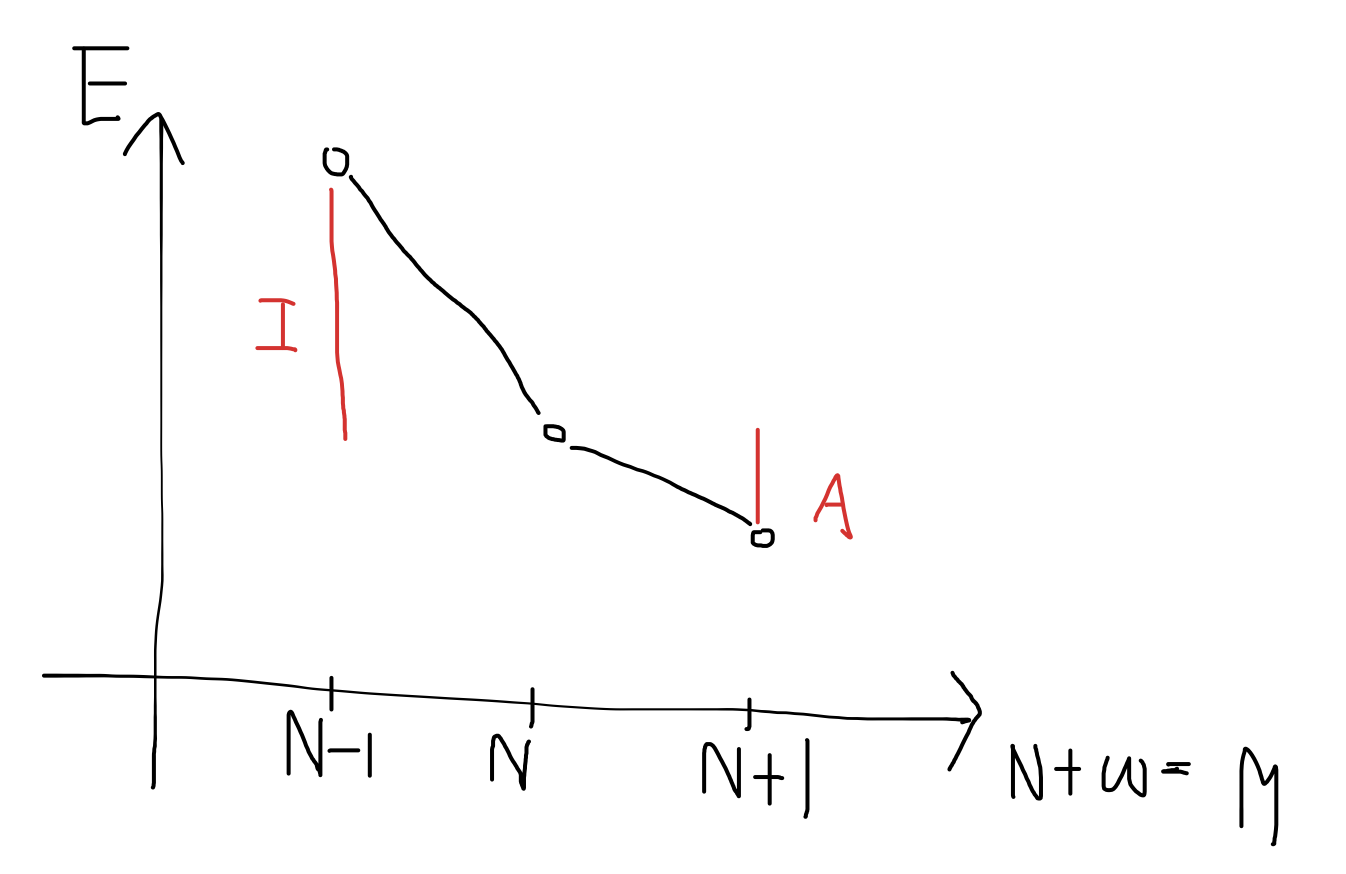
\includegraphics[width=0.5\linewidth]{graph_2.png}
    \caption{Energy vs fractional number of electron}
    \label{fig:fig_2}
\end{figure}

\subsection{DFT and the bandgap problem}
\begin{align}
    \frac{\partial E}{\partial M}=\frac{\partial E[\rho]}{\delta\rho}=\lambda=\mu\\
    \mu=\begin{dcases}
    -I=\varepsilon_N(N-\delta),N-1<M<N\\
    -A=\varepsilon_{N+1}(N+\delta), N<M<N+1
    \end{dcases}
\end{align}

\begin{figure}[t]
    \centering
    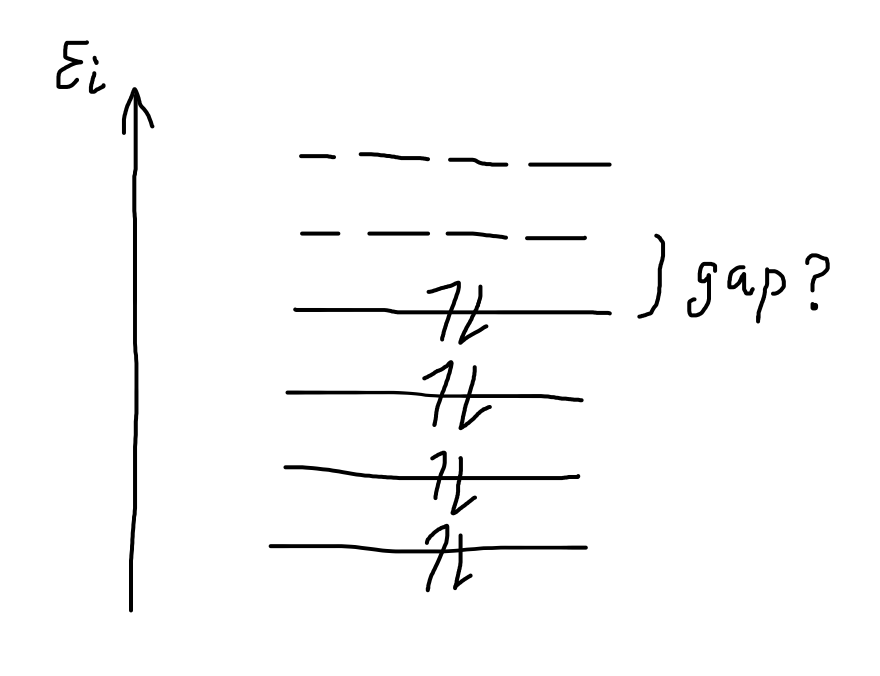
\includegraphics[width=0.5\linewidth]{graph_3.png}
    \caption{}
    \label{fig:figure_3}
\end{figure}

For the real N-electron system:
\begin{align}
    \Delta f &= I-A\\
    &= \frac{\delta E[\rho]}{\delta \rho}\bigg\vert_{N+\delta} - \frac{\delta E[\rho]}{\delta \rho} \bigg\vert_{N-\delta} \qquad \delta\rightarrow0^+\\
    &= \frac{\delta T_{s}[\rho]}{\delta \rho}\bigg\vert_{N+\delta} - \frac{\delta T_{s}[\rho]}{\delta \rho} + \cancelto{0}{V_{ext}\vert_{N+\delta} - V_{ext} \vert_{N-\delta}}\nonumber\\
    &+ \cancelto{0}{e^2\int\frac{\rho(r')}{\abs{\vec{r}-\vec{r'}}}d\vec{r'}\bigg\vert_{N+\delta} - e^2\int\frac{\rho(r')}{\abs{\vec{r}-\vec{r'}}}d\vec{r'}\bigg\vert_{N-\delta}}\nonumber\\
    \nonumber\\
    &+ V_{XC}\vert_{N+\delta}-V_{XC}\vert_{N-\delta}
\end{align}

But the external potential and Hartree energy are continuous, so the discontinuity comes from kinetic energy and exchange correlation energy.


\begin{align}
    \Delta f &= I-A \\
    &= \underbrace{\varepsilon_{N+1}(N+\delta)-\varepsilon_N(N+\delta)}_{\Delta_{KS}} + \underbrace{\varepsilon_{N}(N+\delta)-\varepsilon_{N}(N-\delta)}_{\neq 0}
\end{align}

%The KS-equation can be written as:
%\begin{align}
%    \left(-\frac{\hbar^2}{2m}\nabla^2 + V_{\text{ext}}^{\sigma}(\vec{r})+V_{\text{Hartree}}(\vec{r})+V^{\sigma}_{XC}(\vec{r}) \right)\varphi_i = \varepsilon_i \varphi_i
%\end{align}

Substitute $N=\delta$ and $N-\delta$ on both side and substract the two equation, we can get $\Delta_{XC}=\varepsilon_{N}(N+\delta)-\varepsilon_{N}(N-\delta)$. Therefore, the second term is discontinuity in exchange correlation.

We also have:
\begin{align}
    \Delta_{XC}=V_{XC}\vert_{N+\delta} - V_{XC}\vert_{N-\delta}
    \Delta_{KS}=\frac{\delta T_{s}[\rho]}{\delta \rho}\bigg\vert_{N+\delta} - \frac{\delta T_{s}[\rho]}{\delta \rho}\bigg\vert_{N-\delta}
\end{align}

Noted that $E_{XC}$ cannot be an explicit and differentiable functional of $\rho$.

%\begin{figure}
%    \centering
%    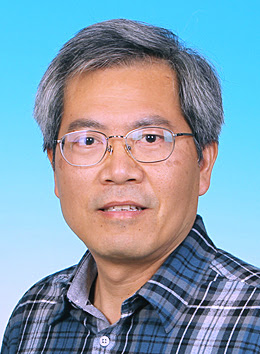
\includegraphics[width=0.3\linewidth]{unnamed.jpg}
%    \caption{A picture of KS}
%    \label{fig:KS}
%\end{figure}

% \begin{figure}
%     \centering
%     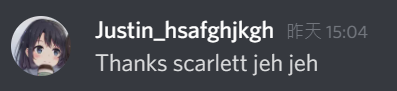
\includegraphics[width=0.5\linewidth]{unknown.png}
%     \caption{Scarlett jeh jeh}
%     \label{fig:siu_sei}
% \end{figure}

\newpage

\chapter{周期固体、基组与赝势}
\sourcepages{原英文稿第 10 章；朋友的 50 页笔记未覆盖本章}
\section{平移对称性如何减少未知量}
晶体有无限多个原胞，逐原子求解不可行。设原胞平移向量为 $\bm a_1,\bm a_2,\bm a_3$，晶格向量为 $\bm R=\sum_i n_i\bm a_i$，有效势满足 $v(\bm r+\bm R)=v(\bm r)$。定义平移算符 $T_R\psi(\bm r)=\psi(\bm r+\bm R)$。势的周期性以及动能的平移不变性给出 $[H,T_R]=0$。对易来自 Hamilton 算符的对称性，不能仅由 $T_R$ 是酉算符推出。

在共同本征态上写 $T_R\psi=t_R\psi$。酉性保证 $|t_R|=1$，群乘法 $T_RT_{R'}=T_{R+R'}$ 要求本征值满足相同乘法关系，故可写 $t_R=e^{\ii\bm k\cdot\bm R}$。定义 $u_{n\bm k}=e^{-\ii\bm k\cdot\bm r}\psi_{n\bm k}$，立即得到
\begin{equation}
\psi_{n\bm k}(\bm r)=e^{\ii\bm k\cdot\bm r}u_{n\bm k}(\bm r),\qquad u_{n\bm k}(\bm r+\bm R)=u_{n\bm k}(\bm r).
\end{equation}
这就是 Bloch 形式，$n$ 标记能带。同一个 Bloch 态的模平方在原胞间相同，但波函数本身一般只差相位，而非严格原胞周期。

倒格矢满足 $\bm a_i\cdot\bm b_j=2\pi\delta_{ij}$。令波函数在 $N_i\bm a_i$ 形成的大超胞上周期，则允许 $\bm k=\sum_i(m_i/N_i)\bm b_i$。相差倒格矢的 $\bm k$ 描述等价平移本征值，故只需第一 Brillouin 区。将 Bloch 形式代入 KS 方程，得到原胞内方程
\begin{equation}
\left[-\tfrac12(\nabla+\ii\bm k)^2+v_s(\bm r)\right]u_{n\bm k}=\varepsilon_{n\bm k}u_{n\bm k}.
\end{equation}
无限晶体问题转化为不同 $\bm k$ 参数下的有限原胞问题。

\section{积分采样与能带路径不是同一件事}
每原胞的 Brillouin 区平均为 $\Omega_{BZ}^{-1}\int_{BZ}A(\bm k)\dd^3k$，其中 $\Omega_{BZ}=(2\pi)^3/\Omega_{\rm cell}$。数值上用 $\sum_k w_kA(\bm k)$，权重和为一。若 $u$ 在原胞归一化，电子密度为 $n(\bm r)=\sum_{nk}w_k f_{nk}|u_{nk}(\bm r)|^2$，自旋简并是否计入 $f$ 必须前后一致。

Monkhorst--Pack 网格的一种写法是 $\bm k=\sum_i(2m_i-N_i-1)\bm b_i/(2N_i)$，$m_i=1,\ldots,N_i$。晶体对称性可把等价点合并，但合并权重必须来自整个离散网格。画能带的高对称路径只是一条线，不能代替三维积分网格。金属的占据在 Fermi 面附近变化快，通常比绝缘体需要更细的采样与展宽收敛检查。

无磁、无自旋轨道耦合且势为实标量时，复共轭把 $\bm k$ 态映为同能量的 $-\bm k$ 态。在合适基中 $\Gamma$ 点可选实轨道。这不意味着所有具有时间反演对称性的系统都有 Dirac 锥；能带交叉还依赖其他对称性和能带结构。含自旋时，时间反演也不能简单等同于复共轭。

\section{平面波为什么方便}
周期函数可展开为 $u_{n\bm k}=\Omega_{\rm cell}^{-1/2}\sum_Gc_{n\bm k}(G)e^{\ii\bm G\cdot\bm r}$。由于 $\nabla e^{\ii G r}=\ii\bm G e^{\ii G r}$、$\nabla^2e^{\ii G r}=-G^2e^{\ii G r}$，动能在倒空间对角。保留 $|\bm k+\bm G|^2/2\le E_{\rm cut}$ 的项，把无限基变成有限基。增大截断在固定几何、嵌套基和充分求解下扩大变分空间，但实际计算还要控制积分网格等误差。

势能乘法在实空间方便，故常以 FFT 在两种表示之间切换。密度包含 $c^*(G)c(G')e^{\ii(G'-G)r}$；若轨道波矢最大为 $G_{\max}$，密度包含至 $2G_{\max}$ 的成分，对应四倍动能截断。这是平面波乘积的几何结论；超软赝势或 PAW 增广密度可能需要更高密度截断，不能机械设成四倍。

Poisson 方程 $\nabla^2v_H=-4\pi n$ 给出 $v_H(G)=4\pi n(G)/G^2$，仅对 $G\ne0$ 成立。电子密度的 $n(0)$ 是平均电子数密度，\emph{不为零}。周期静电的零模需要结合离子电荷、中性条件和势零点约定处理。带电超胞还涉及补偿背景，不能把零模发散解释成分子也变为零。

\section{赝势为何与基组选择相连}
核附近全电子轨道快速变化，并与芯态正交；直接用平面波表示需很高截断。赝势在芯区内用平滑价态与有效作用替代显式芯电子，同时希望保持芯区外的散射性质。对某个角动量通道，模守恒构造要求参考能量和芯区外径向函数匹配，并满足
\begin{equation}
\int_0^{r_c}|R_l(r)|^2r^2\dd r=\int_0^{r_c}|\widetilde R_l(r)|^2r^2\dd r.
\end{equation}
这是约束之一，不是“任意平滑后就等价”的保证。不同角动量需要不同作用，因而赝势一般包含非局域投影项。可转移性必须在不同价态、成键和压强环境中检验。

局域原子轨道基则以较少函数描述成键，但需要控制基组完备性与近线性相关。Slater 型径向函数有 $e^{-\zeta r}$ 的衰减，Gaussian 型用多项式乘 $e^{-\alpha r^2}$，便于积分运算。移动原子会移动局域基，所以力中要考虑第四章的 Pulay 项。实空间有限差分是另一种选择，例如 $\partial_x^2\psi\simeq[\psi(x+a)-2\psi(x)+\psi(x-a)]/a^2$；其网格误差需单独收敛，通常不具有相同的严格变分单调性。

\section{从能带曲率理解有效质量}
在波包半经典近似下，群速度为 $v_\alpha=\hbar^{-1}\partial\varepsilon/\partial k_\alpha$，外力满足 $\hbar\dot k_\beta=F_\beta$。对速度再求时间导数，得到
\begin{equation}
\dot v_\alpha=\sum_\beta\frac1{\hbar^2}\frac{\partial^2\varepsilon}{\partial k_\alpha\partial k_\beta}F_\beta,
\qquad (m^{*-1})_{\alpha\beta}=\frac1{\hbar^2}\frac{\partial^2\varepsilon}{\partial k_\alpha\partial k_\beta}.
\end{equation}
有效质量是带边曲率张量，不是先验输入来决定能带。仅在各向同性抛物线附近，才可简化成一个标量 $m^*$。

\chapter{从势能曲率到晶格振动}
\sourcepages{原英文稿第 11 章；朋友的 50 页笔记未覆盖本章}
\section{平衡结构附近的第一个非平凡近似}
电子结构给出核构型的能量 $E(R)$，但一个极小值只告诉我们原子平均停在哪里。温度与零点运动使原子在附近振动，振动频率由势能曲率决定。设平衡位置为 $R^0$，位移为 $u_{I\alpha}=R_{I\alpha}-R^0_{I\alpha}$。平衡要求一阶导数为零，故
\begin{equation}
E=E_0+\frac12\sum_{I\alpha,J\beta}C_{I\alpha,J\beta}u_{I\alpha}u_{J\beta}+O(u^3),\quad
C_{I\alpha,J\beta}=\frac{\partial^2E}{\partial R_{I\alpha}\partial R_{J\beta}}.
\end{equation}
$C$ 是力常数矩阵，$C=-\partial F/\partial R$。光滑能量的混合导数相等，使它对称。Newton 方程变成 $M_I\ddot u_{I\alpha}=-\sum_{J\beta}C_{I\alpha,J\beta}u_{J\beta}$。

试取所有原子以同一频率振动，$u_{I\alpha}(t)=U_{I\alpha}e^{-\ii\omega t}$，得 $\omega^2M_IU_{I\alpha}=\sum C_{I\alpha,J\beta}U_{J\beta}$。令 $e_{I\alpha}=\sqrt{M_I}U_{I\alpha}$，便得到普通对称本征问题
\begin{equation}
\sum_{J\beta}D_{I\alpha,J\beta}e_{J\beta}=\omega^2e_{I\alpha},\qquad
D_{I\alpha,J\beta}=\frac{C_{I\alpha,J\beta}}{\sqrt{M_IM_J}}.
\end{equation}
质量加权使相同的势能曲率对重原子产生较低的频率。例如双原子一维弹簧 $E=k(u_1-u_2)^2/2$ 有平移零模和 $\omega^2=k(1/M_1+1/M_2)=k/\mu_{\rm red}$ 的相对振动。

\section{冻结位移如何测出曲率}
所谓冻结声子或有限位移方法，是暂时把一个坐标移开 $\pm\Delta$，分别计算所有原子的力：
\begin{equation}
C_{I\alpha,J\beta}\simeq-\frac{F_{I\alpha}(R^0+\Delta\bm e_{J\beta})-F_{I\alpha}(R^0-\Delta\bm e_{J\beta})}{2\Delta}.
\end{equation}
中心差分截断误差通常为 $O(\Delta^2)$。但若力有误差 $\delta F$，差分误差还含 $O(\delta F/\Delta)$；所以位移越小并非总越好。应收紧电子收敛，比较数个振幅，并先把平衡结构优化到足够小的残余力。

若某本征值 $\omega^2<0$，线性化运动含指数增长而不是振荡，说明该构型在相应方向可能不稳定。很小的负值也可能来自数值误差或不充分收敛，不能只看绘图软件画出的“负频率”就断定新相。

\section{零模数量取决于系统}
孤立非线性分子的整体平移和转动不改变能量，通常有三个平移及三个转动零模，剩 $3N-6$ 个振动模；线性分子只有两个独立转动方向，剩 $3N-5$ 个振动模。固定周期晶胞不能任意刚体转动而保持边界不变，晶体在 $\bm q=0$ 有三个声学平移零模，不能照搬分子的六零模计数。

整体平移使所有原子同向移动，力仍为零，故 $\sum_JC_{I\alpha,J\beta}=0$，称声学和规则。它既是物理约束，也是数值检验；强制修正不能替代检查原始力的收敛。

\section{从超胞力常数到声子}
晶体中以胞标号 $l$ 和胞内原子 $\kappa$ 区分原子。取振动形式 $u_{l\kappa\alpha}=M_\kappa^{-1/2}e_{\kappa\alpha}(\bm q)e^{\ii(\bm q\cdot\bm R_l-\omega t)}$，代入运动方程，得到
\begin{equation}
D_{\kappa\alpha,\kappa'\beta}(\bm q)=\frac1{\sqrt{M_\kappa M_{\kappa'}}}\sum_l C_{0\kappa\alpha,l\kappa'\beta}e^{\ii\bm q\cdot\bm R_l}.
\end{equation}
超胞决定可可靠恢复的作用距离；极性材料的长程偶极作用还需处理非解析修正。本式采用只在胞向量上带相位的约定，其他加入胞内坐标的约定给出等价频率。

上述正则模可以用经典力学求频率，但声子是它们量子化后的激发。每个独立模的能级为 $\hbar\omega(n+1/2)$，因此即使零温也有零点能。有限温谐振动自由能为
\begin{equation}
F_{\rm vib}=\sum_{\bm q\nu}\left[\frac{\hbar\omega_{\bm q\nu}}2+\kb T\ln(1-e^{-\beta\hbar\omega_{\bm q\nu}})\right],
\end{equation}
其中求和按所需总量或每胞量归一化，刚体零模需另行处理。高温才恢复每模平均能量约 $\kb T$ 的经典极限。因此“频率由经典方程求出”不等于“声子没有量子性”。

\chapter{让电子变量与原子核一起推进}
\section{Born--Oppenheimer 动力学的计算负担}
Born--Oppenheimer 动力学在每个新核构型都须先求解电子基态，再求力、推进核。Car--Parrinello 方法让轨道沿着随核移动的能量最低点附近连续演化，以减少逐步从头最小化的工作。

这里的轨道运动是辅助数值动力学，不是实际电子的含时 Schrödinger 演化。下面为清楚起见采用固定单占据的正交自旋轨道；闭壳层双占据形式须一致地处理占据系数。

\section{扩展 Lagrange 函数与约束}
保留真实核动能，以电子能量泛函作为势能，再给轨道速度添加正的二次项，其系数 $\mu$ 是可选择的虚拟惯性参数。用乘子加入轨道正交约束，定义扩展 Lagrange 函数
\begin{equation}
L=\frac12\sum_I M_I|\dot{\bm R}_I|^2+
\mu\sum_i\langle\dot\phi_i|\dot\phi_i\rangle-E[\{\phi\},R]
+\sum_{ij}\Lambda_{ij}(\langle\phi_i|\phi_j\rangle-\delta_{ij}).
\end{equation}
两个动能项都带正号，核动能含速度平方。$\mu$ 的量纲使 $\mu\langle\dot\phi|\dot\phi\rangle$ 为能量；它不是电子的真实质量。本章取复轨道约定，不在该项前再放 $1/2$。

对每个坐标重复第一章作用量变分中的分部积分，端点变化为零后，任意内部路径变化的系数必须为零。这给出 Euler--Lagrange 方程
\begin{equation}
\frac{\dd}{\dd t}\frac{\partial L}{\partial\dot q}=\frac{\partial L}{\partial q}.
\end{equation}
对核坐标，$\partial L/\partial\dot{\bm R}_I=M_I\dot{\bm R}_I$；假设基组不随核移动，则固定轨道时的约束项不含核坐标，$\partial L/\partial\bm R_I=-\partial E/\partial\bm R_I$。因此
\begin{equation}
M_I\ddot{\bm R}_I=-\frac{\partial E}{\partial\bm R_I}.
\end{equation}
对 $\phi_i^*$ 作独立变分，$\delta L/\delta\dot\phi_i^*=\mu\dot\phi_i$，而 $\delta L/\delta\phi_i^*=-\delta E/\delta\phi_i^*+\sum_j\Lambda_{ij}\phi_j$。把二者代入同一 Euler--Lagrange 方程，再使用第七章已推导的单占据轨道能量导数 $\delta E/\delta\phi_i^*=\hat H_{\rm KS}\phi_i$，得到
\begin{equation}
\mu\ddot\phi_i=-\frac{\delta E}{\delta\phi_i^*}+\sum_j\Lambda_{ij}\phi_j
=-\hat H_{\rm KS}\phi_i+\sum_j\Lambda_{ij}\phi_j.
\end{equation}
乘子矩阵取 Hermitian 形式，使约束项为实数并维持轨道正交。静止时的驻值方程可经占据子空间酉变换化为 KS 本征方程；传播中的轨道则未必是瞬时基态。

守恒量也应从这个辅助 Lagrange 函数推导。把核坐标、轨道的实部与虚部以及约束乘子合并记为广义坐标 $q_a$，定义 $\mathcal E=\sum_a\dot q_a\partial L/\partial\dot q_a-L$。逐项求时间导数，含 $\ddot q_a$ 的项抵消，得到
\begin{equation}
\frac{\dd\mathcal E}{\dd t}
=\sum_a\dot q_a\left[\frac{\dd}{\dd t}\frac{\partial L}{\partial\dot q_a}
-\frac{\partial L}{\partial q_a}\right]-\frac{\partial L}{\partial t}=0.
\end{equation}
最后一步用了运动方程及没有显式时间依赖。核与轨道的速度项都是二次齐次函数，所以 $\sum_a\dot q_a\partial L/\partial\dot q_a$ 等于它们的两倍；减去 $L$ 后，各留下一个正的动能项，并加回电子势能。约束项在 $\langle\phi_i|\phi_j\rangle=\delta_{ij}$ 时为零，乘子本身也没有速度项。因此连续精确动力学守恒的量是
\begin{equation}
E_{\rm ext}=\frac12\sum_I M_I|\dot{\bm R}_I|^2+
\mu\sum_i\langle\dot\phi_i|\dot\phi_i\rangle+E[\{\phi\},R].
\end{equation}
这不等于物理核动能加 BO 基态能量：虚拟电子动能也包含其中。数值积分还会带误差。仅见 $E_{\rm ext}$ 近似守恒，不能证明核始终在正确的基态面上运动。

\section{两能级模型解释频率分离}
固定核，令 $H|1\rangle=\varepsilon_1|1\rangle$、$H|2\rangle=\varepsilon_2|2\rangle$，$\Delta=\varepsilon_2-\varepsilon_1>0$。以归一化试探态 $|\phi\rangle=\cos(\theta/2)|1\rangle+\sin(\theta/2)|2\rangle$ 描述偏离基态的程度。求导得 $|\dot\phi\rangle=(\dot\theta/2)[-\sin(\theta/2)|1\rangle+\cos(\theta/2)|2\rangle]$。由两态正交性，速度范数中的交叉项为零，余下 $\dot\theta^2[\sin^2(\theta/2)+\cos^2(\theta/2)]/4$。能量期望值同样只有 $\varepsilon_1\cos^2(\theta/2)+\varepsilon_2\sin^2(\theta/2)$；使用 $\cos^2=1-\sin^2$，两者分别成为
\begin{equation}
\langle\dot\phi|\dot\phi\rangle=\dot\theta^2/4,\qquad
\langle\phi|H|\phi\rangle=\varepsilon_1+\Delta\sin^2(\theta/2).
\end{equation}
因此 $L=\mu\dot\theta^2/4-\varepsilon_1-\Delta\sin^2(\theta/2)$。逐项求导有
\begin{equation}
\frac{\partial L}{\partial\dot\theta}=\frac\mu2\dot\theta,\qquad
\frac{\partial L}{\partial\theta}=-\Delta\sin\frac\theta2\cos\frac\theta2
=-\frac\Delta2\sin\theta.
\end{equation}
Euler--Lagrange 方程成为 $(\mu/2)\ddot\theta=-(\Delta/2)\sin\theta$。小振幅时用 $\sin\theta=\theta+O(\theta^3)$，再除以 $\mu/2$；试取 $\theta\propto e^{\ii\omega_et}$，有 $-\omega_e^2+\Delta/\mu=0$。故
\begin{equation}
\ddot\theta+(\Delta/\mu)\theta=0,\qquad \omega_e=\sqrt{\Delta/\mu}.
\end{equation}
若电子辅助振动远快于核振动且初始激发很小，轨道有可能保持在移动最低点附近。降低 $\mu$ 增大频率分离，却也要求更小时间步。能隙小的金属使这一分离困难，不能把该方法视为对任意体系都自动成立的加速器。

\section{实际可信性要检验什么}
用类似 Verlet 的方法推进时，须同时求解轨道正交约束；逐条归一化不能保证相互正交，也可能破坏可逆性。应检查正交残差、扩展能量漂移、虚拟电子动能是否持续升高，以及目标量对 $\mu$ 和步长的收敛。抽取核构型重新求电子基态，若 CP 能量与 BO 能量之差随时间增大，就说明轨道逐渐偏离基态面。还须对照收敛的 BO 力或轨迹统计量，检验辅助动力学对核运动的影响。

\end{document}
